\chapter{Σχεδίαση εφαρμογής}\label{chapter:3-application-design}

Σε αυτό το κεφάλαιο περιγράφεται η διαδικασία σχεδίασης της εφαρμογής Concordia, από τη σύλληψη της ιδέας και την επιλογή της τεχνολογικής στοίβας, μέχρι τον ορισμό της αρχιτεκτονικής της και τον διαχωρισμό του προγραμματιστικού έργου σε sprints. 

\section{Σύλληψη της ιδέας} \label{section:3-1-idea-conception}

\section{Τεχνολογική στοίβα} \label{section:3-2-technology-stack}

Ξεκινώντας τη σχεδίαση της πλατφόρμας, πραγματοποιήθηκε έρευνα για την επιλογή της τεχνολογικής της στοίβας (technology stack). Αυτή αποφασίστηκε να ακολουθήσει μία προσαρμοσμένη για τα δεδομένα μορφή τριμερούς διάταξης\footnote{Η τριμερής διάταξη (three-tier architecture) διαχωρίζει μία εφαρμογή σε τρία ανεξάρτητα λειτουργικά επίπεδα και αποτελεί την κυρίαρχη επιλογή για διατάξεις παραδοσιακών εφαρμογών πελάτη-εξυπηρετητή.} και να χωριστεί σε τρία λογικά επίπεδα (tiers):

\begin{enumerate}
    \item \textbf{Presentation tier}: Αποτελεί τη διεπαφή του χρήστη (user interface ή UI), μέσω της οποίας ο τελευταίος αλληλεπιδρά με την εφαρμογή. Για την εκπλήρωση των προδιαγραφών, το μοναδικό απαραίτητο χαρακτηριστικό αυτού του τμήματος είναι να μπορεί να εκτελείται αυτούσιο από τη συσκευή του τελικού χρήστη, δηλαδή να μην απαιτείται η ύπαρξη κάποιου εξυπηρετητή για τη λειτουργία του. Λαμβάνοντας, επιπροσθέτως, υπόψιν τις ανάγκες και τους περιορισμούς των λογισμικών των άλλων δύο επιπέδων, το παρόν κομμάτι αποφασίστηκε να σχεδιαστεί ως μία client-side web application σε HTML/CSS/JavaScript.

    \item \textbf{Application tier}: Πρόκειται για το επίπεδο που πραγματοποιεί την επεξεργασία (\textenglish{processing}) της εφαρμογής. Εδώ επιλέχθηκαν το blockchain και τα smart contracts, καθώς τα πλεονεκτήματά τους, όπως αυτά περιγράφηκαν στο κεφάλαιο \ref{chapter:2-theoretical-background}, αρμόζουν απόλυτα με τις ιδιαίτερες απαιτήσεις της εφαρμογής. Συγκεκριμένα, επιλέχθηκε η πλατφόρμα του Ethereum, καθώς αποτελεί τον πρωτοπόρο στο χώρο, διαθέτοντας την ισχυρότερη κοινότητα και την δυνατότητα δημιουργίας πλήρως λειτουργικών εφαρμογών.

    \item \textbf{Data tier}: Το τμήμα αυτό είναι υπεύθυνο για την αποθήκευση του κύριου όγκου των δεδομένων (storage). Για την επίτευξη πλήρους αρχιτεκτονικής αποκέντρωσης των δεδομένων επιλέχθηκε το IPFS (βλ. ενότητα \ref{section:2-7-ipfs}), το οποίο διανέμει το περιεχόμενο της εφαρμογής στους peers που συμμετέχουν σε αυτήν, χωρίς να απαιτεί κάποιο κεντρικό σημείο. Έτσι, κάθε χρήστης θα έχει πλήρη κυριότητα επί των δεδομένων του, ενώ, επιπλέον, θα συμμετέχει στην πλατφόρμα διαμοιράζοντας τα δεδομένα άλλων χρηστών.
\end{enumerate}

Τελικά, με τη διασύνδεση των προαναφερθέντων τεχνολογιών, προκύπτει σχηματικά η ακόλουθη διάταξη:

\begin{figure}[H]
    \centering
    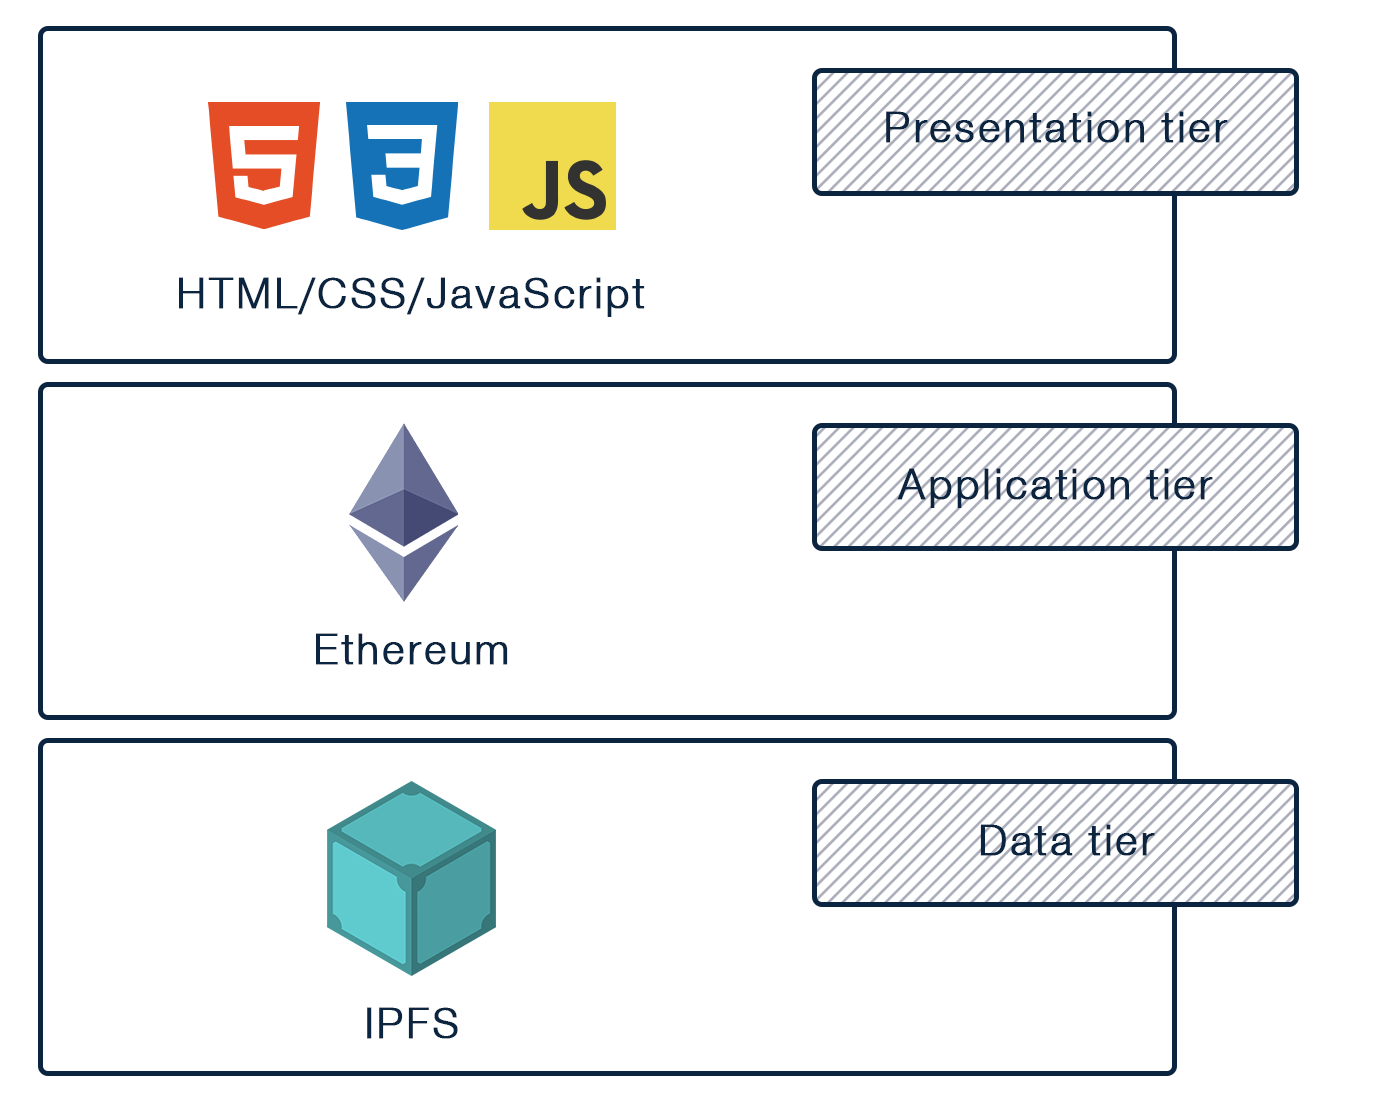
\includegraphics[width=.55\textwidth]{assets/figures/chapter-3/3.2.technology.stack}
    \caption{Επιλεγμένη τεχνολογική στοίβα}
\end{figure}

\section{Μεθοδολογία σχεδίασης} \label{section:3-3-design-methodology}

Στον χώρο της τεχνολογίας λογισμικού υπάρχουν διάφορες μεθοδολογίες σχεδίασης οι οποίες έχουν μεταξύ τους κοινά στοιχεία. Αυτό καθιστά δύσκολο τον προσδιορισμό μίας μόνο μεθοδολογίας η οποία ακολουθείται πιστά σε κάθε έργο. Συνήθως, οι ομάδες που αναπτύσσουν το λογισμικό ακολουθούν μία μίξη από διάφορα εργαλεία, όπου αυτά κρίνονται βολικά για τους στόχους της ομάδας. % todo: need reference for this

Κατά την σχεδίαση και την υλοποίηση του κώδικα ακολουθήθηκαν διάφορες τεχνικές και μοτίβα ανάπτυξης. Κατά βάση χρησιμοποιήθηκαν Agile μέθοδοι όπως το Kanban και Scrum και, αργότερα στην ανάπτυξη, το DevOps μοντέλο για διαρκή ενσωμάτωση (Continuous Integration) και διαρκή εγκατάσταση (Continuous Deployment).

% todo: add an intro to agile too?

Για την παρούσα εργασία, πραγματοποιήθηκε ανάλυση και σχεδιασμός των επιμέρους μονάδων εργασίας (tasks) πριν την έναρξη της διαδικασίας ανάπτυξης του κώδικα. Τα tasks που προδιαγράφηκαν ήταν συνήθως epics\footnote{Τα epics είναι μεγάλες μονάδες εργασίας οι οποίες αφορούν κάποιο βασικό χαρακτηριστικό. Ο διαχωρισμός τους σε επιμέρους tasks αναβάλλεται με σκοπό την καλύτερη κατανόηση των αναγκών τους.} τα οποία αργότερα χωρίστηκαν σε επιμέρους, μικρότερα tasks. Ορίστηκαν επίσης ορόσημα (milestones) τα οποία βοήθησαν ιδιαίτερα στην ιεράρχηση και προτεραιοποίηση των tasks.

Το Kanban είναι μία μέθοδος οργάνωσης έργων και οπτικοποίησης των μονάδων εργασίας (tasks) που απαιτούνται για την ολοκλήρωσή τους. Στο Kanban ορίζονται τα βασικά στάδια της ροής ενός task και χρησιμοποιούνται οπτικά μέσα ώστε να γίνει ιχνηλάτηση τόσο της συνολικής κατάστασης του έργου, όσο και συγκεκριμένων-μεμονωμένων tasks καθώς αυτά προοδεύουν. Για κάθε στάδιο ολοκλήρωσης ορίζεται μία ξεχωριστή ουρά εργασιών (στήλη), για παράδειγμα "σε αναμονή", "σε εξέλιξη", "ολοκληρωμένο". Χρησιμοποιούνται οπτικά σινιάλα (χρώματα, tags και άλλα) για τον διαχωρισμό και την γρήγορη κατανόηση των σημαντικότερων γνωρισμάτων των tasks, για παράδειγμα ξεχωριστό tag για κάθε υπηρεσία στην οποία αναφέρεται το task. Επίσης, ορίζονται όρια στον αριθμό των tasks που μπορούν να είναι ταυτόχρονα σε εξέλιξη.

Μία άλλη Agile μέθοδος είναι το SCRUM. Το SCRUM χρησιμοποιεί και επεκτείνει το Kanban. Η βασικές διαφορές του με το Kanban είναι ότι στο SCRUM υπάρχουν πιο αυστηρές διαδικασίες. Ορίζονται προγραμματιστικοί κύκλοι (sprints) οι οποίοι έχουν συγκεκριμένες ημερομηνίες έναρξης και λήξης και συγκεκριμένους στόχους οι οποίοι αντικατοπτρίζονται σε στόχους ολοκλήρωσης ορισμένων tasks. Οι ρόλοι είναι σαφέστεροι, με κάθε μέλος της ομάδας να αναλαμβάνει διαφορετικές ευθύνες στην οργάνωση και εκτέλεση. Για την διαδικασία ανάπτυξης, υπήρξε πολύ χρήσιμη η χρήση του SCRUM σε περιόδους όπου ήταν αναγκαία η ταχύτατη ανάπτυξη καίριων μερών του συστήματος. Λόγω της αυστηρότητας που επιβάλλεται από αυτό, ειδικά σε ό,τι αφορά τις προθεσμίες ολοκλήρωσης των επιμέρους tasks αλλά και του συνολικού sprint.

Καθώς η αναπτυξιακή διαδικασία ωριμάζει και η πλατφόρμα αποτελεί ένα βιώσιμο προϊόν, είναι χρήσιμη η ύπαρξη ενός συστήματος που να διευκολύνει την άμεση δημιουργία και δημοσίευση των νεότερων εκδόσεων. Μερικές εξαιρετικές μέθοδοι για την απρόσκοπτη και αυτοματοποιημένη επίτευξη του στόχου αυτού ορίζονται από το DevOps. Με τον όρο DevOps (development operations) αναφέρεται μία κουλτούρα σχεδίασης και ανάπτυξης λογισμικού που ορίζει τους ρόλους, τις διαδικασίες και τεχνολογίες της με σκοπό την συνεχή δημιουργία αξίας για τους χρήστες. Το DevOps έχει πολύ στενή σχέση με το Agile και αποτελεί την συνέχιση της νοοτροπίας αυτής στον χώρο.

Μία από τις πιο χρήσιμες πτυχές του DevOps, η οποία χρησιμοποιήθηκε στην διπλωματική, είναι το CI/CD το οποίο περιγράφει τις διαδικασίες αυτοματοποίησης των εργασιών ενσωμάτωσης (integration), ελέγχου (testing), παράδοσης (delivery) και εγκατάστασης (deployment) του προϊόντος. Μέσω των διαδικασιών αυτών αφαιρείται η ανάγκη ανθρώπινης αλληλεπίδρασης για την ολοκλήρωση των σταδίων αυτών, ενώ επιτυγχάνεται η διαρκής και απρόσκοπτη διάθεση της τελευταίες έκδοσης της πλατφόρμας στους χρήστες. Ορίζονται επίσης διαδικασίες δημιουργίας περιβάλλοντος ελέγχου (staging deploys) το οποίο αποτελεί σημαντικό βοήθημα στον έγκαιρο εντοπισμό λαθών του κώδικα.

\section{Κατηγορίες χρηστών} \label{section:3-4-user-categories}

Οι χρήστες (actors) της πλατφόρμας χωρίζονται σε πρωτεύοντες ή ενεργούς και δευτερεύοντες ή παθητικούς. Πρωτεύοντες χρήστες είναι εκείνοι που εκκινούν διεργασίες στο σύστημα. Δευτερεύοντες είναι οι χρήστες με τους οποίους αλληλεπιδρά το σύστημα, αλλά οι ίδιοι δεν εκκινούν διεργασίες σε αυτό. Συνολικά οι χρήστες που συμμετέχουν στο σύστημα είναι οι:

\begin{itemize}
    \item Επισκέπτες
    \item Εγγεγραμμένα μέλη
    \item Συμβόλαια κοινοτήτων
\end{itemize}

\subsection{Ενεργοί χρήστες}

Οι ενεργοί χρήστες στο σύστημα είναι οι επισκέπτες και τα εγγεγραμμένα μέλη.

Όλοι οι χρήστες στο σύστημα είναι αρχικά επισκέπτες. Οι επισκέπτες έχουν τη δυνατότητα να βλέπουν το περιεχόμενο της κοινότητας, αλλά δε μπορούν να συμμετέχουν δημιουργώντας νέο περιεχόμενο (δημοσιεύοντας νέα θέματα ή μηνύματα). Επίσης, δε μπορούν να συμμετέχουν στις ψηφοφορίες της κοινότητας ή να ψηφίσουν τα μηνύματα.

Όταν ένας επισκέπτης εγγράφεται στο σύστημα, αποκτά έναν μοναδικό, αύξοντα αριθμό χρήστη και αποτελεί πλέον εγγεγραμμένο μέλος της κοινότητας. Τα εγγεγραμμένα μέλη έχουν τα δικαιώματα των επισκεπτών και μπορούν επιπλέον να προσθέσουν περιεχόμενο στην πλατφόρμα μέσω της δημιουργίας νέων θεμάτων, της δημοσίευσης μηνυμάτων και της ψήφισης στις ψηφοφορίες στις οποίες έχουν δικαίωμα.

\subsection{Παθητικοί χρήστες}

Παθητικοί χρήστες τους συστήματος είναι τα συμβόλαια των κοινοτήτων. Τα συμβόλαια αυτά δεν εκκινούν διεργασίες στο σύστημα και δεν αλληλεπιδρούν με αυτό άμεσα. Αποτελούν αυτόνομες εξωτερικές οντότητες, οι οποίες ορίζουν τους χρήστες κοινοτήτων μέσω της διάθεσης αναγνωριστικών token στα μέλη τους. Συγκεκριμένα, μέσω του διαμοιρασμού των token, καθορίζουν ποιοι χρήστες της πλατφόρμας έχουν δικαίωμα ψήφου στις ψηφοφορίες που αφορούν την κοινότητα.

\subsection{Σύνοψη χρηστών}

Συμπερασματικά προκύπτουν δύο διακριτές κατηγορίες ενεργών χρηστών με ξεχωριστά δικαιώματα όπως φαίνεται στο παρακάτω σχήμα:

\begin{threeparttable}[H]
    \begin{center}
        \begin{tabularx}{\textwidth}{p{2.3cm} X X X X X X X X X}
            \toprule
            \multirow{7}{2.3cm}{\textbf{Κατηγορία χρήστη}} &\multicolumn{9}{c}{\textbf{Δικαιώματα}} \\ [0.5ex]
            & \spheading{70}{6em}{Προβολή θεμάτων} & \spheading{70}{8em}{Προβολή μηνυμάτων} & \spheading{70}{8em}{Προβολή ψηφοφοριών} & \spheading{70}{8em}{Προβολή ψήφων μηνυμάτων} & \spheading{70}{8em}{Δημιουργία θεμάτων} & \spheading{70}{8em}{Δημιουργία μηνυμάτων} & \spheading{70}{8em}{Δημιουργία ψηφοφοριών} & \spheading{70}{8em}{Ψήφιση σε ψηφοφορίες} & \spheading{70}{8em}{Ψήφιση μηνυμάτων} \\ [0.5ex]
            \midrule
            Επισκέπτες & \ \textcolor{OliveGreen}{\faIcon{check}} & \ \textcolor{OliveGreen}{\faIcon{check}} & \ \textcolor{OliveGreen}{\faIcon{check}} & \ \textcolor{OliveGreen}{\faIcon{check}} & \ \textcolor{red}{\faIcon{times}} & \ \textcolor{red}{\faIcon{times}} & \ \textcolor{red}{\faIcon{times}} & \ \textcolor{red}{\faIcon{times}} & \ \textcolor{red}{\faIcon{times}} \\ [0.5ex]
            Εγγεγραμμένα μέλη & \ \textcolor{OliveGreen}{\faIcon{check}} & \ \textcolor{OliveGreen}{\faIcon{check}} & \ \textcolor{OliveGreen}{\faIcon{check}} & \ \textcolor{OliveGreen}{\faIcon{check}} & \ \textcolor{OliveGreen}{\faIcon{check}} & \ \textcolor{OliveGreen}{\faIcon{check}} & \ \textcolor{OliveGreen}{\faIcon{check}}\tnote{*} & \ \textcolor{OliveGreen}{\faIcon{check}}\tnote{*} & \ \textcolor{OliveGreen}{\faIcon{check}} \\ [0.5ex]
            \bottomrule
        \end{tabularx}
        \begin{tablenotes}
            \item[*] \footnotesize{Μόνο στις κοινότητες στις οποίες κατέχει το αντίστοιχο token και σε αυτές οι οποίες δεν έχουν ορισμένο token.}
        \end{tablenotes}
    \end{center}
    \caption{Δικαιώματα χρήσης ανά κατηγορία χρήστη}
    \label{table:3-4-user-category-permissions}
\end{threeparttable}

\section{Απαιτήσεις λογισμικού} \label{section:3-5-software-requirements}

Στην παρούσα ενότητα περιγράφονται οι βασικές απαιτήσεις λογισμικού ( \textenglish{software requirements}) της εφαρμογής.

Η πρώτη κατηγορία είναι αυτή των Λειτουργικών Απαιτήσεων (ΛΑ), η οποία αναφέρεται στη συμπεριφορά του συστήματος, δηλαδή στον τρόπο που θα αντιδρά και στις εξόδους που θα παράγει ανάλογα με τις εισόδους.

\begin{enumerate}[label=\textbf{<ΛΑ-\arabic*>}, leftmargin=\parindent, align=left, labelwidth=\parindent, labelsep=0pt]
	\sysReqItem
		{\label{srs:functional-srs-sign-up}}
		{Ο χρήστης πρέπει να μπορεί να εγγραφεί στην εφαρμογή με τον Ethereum λογαριασμό του.}
		{Ο χρήστης πρέπει να μπορεί να εγγραφεί στην εφαρμογή, πατώντας το κουμπί "Sign Up" και συμπληρώνοντας τα απαραίτητα πεδία σύμφωνα με τις οδηγίες. Το πεδίο "Username" είναι υποχρεωτικό να συμπληρωθεί με το επιθυμητό username, το οποίο ορίζεται με μοναδικό τρόπο. Σε περίπτωση που ο χρήστης εισάγει μη διαθέσιμο Username, το σύστημα θα πρέπει να μην επιτρέπει στον χρήστη να συνεχίσει και να προβάλει αντίστοιχο μήνυμα λάθους. Επιπλέον, υπάρχουν τα προαιρετικά πεδία "Profile picture URL" και "Location", στα οποία ο χρήστης μπορεί να εισάγει μία εικόνα προφίλ και την τοποθεσία του αντίστοιχα.}
		{5}{Η απαίτηση είναι ύψιστης προτεραιότητας για τους επισκέπτες, καθώς μόνο μέσω της εγγραφής μπορούν να χρησιμοποιήσουν τα υπόλοιπα χαρακτηριστικά της εφαρμογής (όπως φαίνεται στον πίνακα \ref{table:3-4-user-category-permissions}).}
		{5}{Η απαίτηση είναι ύψιστης σημασίας για το σύστημα, επειδή επηρεάζει τη λειτουργικότητά του.}

	\sysReqItem
		{\label{srs:functional-srs-sign-in}}
		{Ο χρήστης πρέπει να μπορεί συνδέεται στην εφαρμογή, εφόσον είναι εγγεγραμμένος.}
		{Το σύστημα πρέπει να διαπιστώνει αυτόματα εάν το τρέχον Ethereum address έχει λογαριασμό στην εφαρμογή και εάν ναι, να συνδέει να τον χρήστη, ανακτώντας το Username του από το blockchain και προβάλλοντας το στο μενού.}
		{5}{Αυτή η απαίτηση είναι ύψιστης προτεραιότητας για τους χρήστες, καθώς μέσω της σύνδεσης ενεργοποιούνται τα χαρακτηριστικά της δημιουργίας θεμάτων και δημοσίευσης μηνυμάτων.}
		{5}{Η απαίτηση είναι ύψιστης σημασίας για το σύστημα, επειδή επηρεάζει τη λειτουργικότητά του.}

	\sysReqItem
		{\label{srs:functional-srs-create-user-databases}}
		{Το σύστημα πρέπει να δημιουργεί τις απαραίτητες βάσεις δεδομένων και να τις συγχρονίζει με το δίκτυο.}
		{Το σύστημα πρέπει να δημιουργεί τις απαραίτητες OrbitDB βάσεις δεδομένων, εάν αυτές δεν υπάρχουν ήδη τοπικά. Όταν ο χρήστης ξεκλειδώνει τον Ethereum λογαριασμό του, το σύστημα θα πρέπει να τον προτρέπει να υπογράψει με το ιδιωτικό του κλειδί τη συναλλαγή δημιουργίας της OrbitDB Identity του. Αυτή θα εξασφαλίζει τη γνησιότητα των βάσεών του και των δεδομένων που εκείνες θα περιέχουν. Επιπλέον, τοπικές βάσεις δεδομένων θα πρέπει να συγχρονίζονται με τις βάσεις άλλων IPFS κόμβων και να διατηρούνται ενημερωμένες.}
		{5}{Η απαίτηση αυτή είναι ύψιστης σημασίας για τους χρήστες, καθώς η πλειοψηφία των δεδομένων της εφαρμογής διατηρούνται σε αυτές τις βάσεις.}
		{5}{Η παρούσα απαίτηση είναι ύψιστης σημασίας για το σύστημα, καθώς οι περισσότερες θεμελιώδεις λειτουργίες της εφαρμογής προϋποθέτουν την αποθήκευση δεδομένων σε OrbitDB βάσεις.}

	\sysReqItem
		{\label{srs:functional-srs-create-topic}}
		{Ο εγγεγραμμένος χρήστης πρέπει να μπορεί να δημιουργεί θέματα (topics).}
		{Ο εγγεγραμμένος χρήστης πρέπει να μπορεί να δημιουργεί νέα θέματα. Αυτό το επιτυγχάνει πατώντας το κουμπί "New Topic", συμπληρώνοντας τα υποχρεωτικά πεδία της φόρμας ("Topic subject" και "First post content"), πατώντας το κουμπί "Create Topic" και επιβεβαιώνοντας τη συναλλαγή στο Ethereum.}
		{5}{Αυτή η απαίτηση είναι υψηλής σημασίας καθώς επιτελεί έναν από τους βασικούς στόχους της πλατφόρμας.}
		{5}{Η απαίτηση είναι υψηλής σημασίας για τον ίδιο λόγο.}

	\sysReqItem
		{\label{srs:functional-srs-browse-community-topics}}
		{Ο χρήστης πρέπει να μπορεί να περιηγείται στα θέματα μίας κοινότητας.}
		{Το σύστημα πρέπει να μπορεί να προβάλλει τα δημιουργημένα θέματα μίας κοινότητας στην αρχική οθόνη της. Ο χρήστης πρέπει να μπορεί να περιηγείται σε αυτά πατώντας πάνω τους και, έπειτα, χρησιμοποιώντας τα βέλη πλοήγησης, να περιηγηθεί στο ιστορικό των μηνυμάτων του θέματος.}
		{5}{Η απαίτηση αυτή είναι υψηλής σημασίας, αφού επιτρέπει στους επισκέπτες να έχουν πρόσβαση στο δημοσιευμένο υλικό της πλατφόρμας.}
		{5}{Πρόκετια για απαίτηση υψηλής σημασίας, επειδή αποτελεί βασικό χαρακτηριστικό για τη χρηστικότητα της πλατφόρμας.}

	\sysReqItem
		{\label{srs:functional-srs-create-post}}
		{Ο εγγεγραμμένος χρήστης πρέπει να μπορεί να δημιουργεί μηνύματα (posts).}
		{Ο εγγεγραμμένος χρήστης πρέπει να μπορεί να δημιουργεί μηνύματα στο θέμα που επιθυμεί. Αυτό επιτυγχάνεται συμπληρώνοντας το πεδίο νέου μηνύματος στην οθόνη του θέματος, πατώντας το κουμπί "Post" και επιβεβαιώνοντας τη συναλλαγή στο Ethereum.}
		{5}{Αυτή η απαίτηση είναι ύψιστης σημασίας για τους χρήστες, επειδή αποτελεί ένα από τα βασικότερα χαρακτηριστικά της πλατφόρμας.}
		{5}{Η απαίτηση αυτή είναι ύψιστης σημασίας για το σύστημα, καθώς αποτελεί θεμελιώδες κομμάτι για την επίτευξη του βασικότερου στόχου της, δηλαδή της δημιουργίας διαλόγου.}

	\sysReqItem
		{\label{srs:functional-srs-modify-post}}
		{Ο χρήστης πρέπει να μπορεί να τροποποιεί τα μηνύματά του.}
		{Ο χρήστης πρέπει να μπορεί να τροποποιεί τα μηνύματά του. Αυτό το επιτυγχάνει επιλέγοντας το κουμπί επεξεργασίας στο εκάστοτε μήνυμα, πραγματοποιώντας τις επιθυμητές τροποποιήσεις και πατώντας το κουμπί επιβεβαίωσης. Στη συνέχεια, το σύστημα τροποποιεί το περιεχόμενο του μηνύματος στη βάση δεδομένων του χρήστη. Σε περίπτωση που ο χρήστης αλλάξει γνώμη κατά τη διάρκεια της διαδικασίας της επεξεργασίας, μπορεί να πατήσει το κουμπί ακύρωσης και να αναιρέσει τις αλλαγές που πραγματοποίησε.}
		{4}{Η απαίτηση αυτή αποτελεί σημαντικό χαρακτηριστικό, καθώς παρέχει στους χρήστες άμεσο έλεγχο επί των δεδομένων τους.}
		{3}{Αυτή η απαίτηση είναι μέτριας σημαντικότητας για το σύστημα, επειδή αυτό θα μπορούσε να είναι λειτουργικό χωρίς το χαρακτηριστικό της επεξεργασίας μηνυμάτων.}

	\sysReqItem
		{\label{srs:functional-srs-vote-posts}}
		{Ο εγγεγραμμένος χρήστης πρέπει να μπορεί να ψηφίζει σε μηνύματα άλλων χρηστών.}
		{Ο εγγεγραμμένος χρήστης πρέπει να μπορεί να υπερψηφίζει ή να καταψηφίζει μηνύματα άλλων χρηστών. Αυτό το επιτυγχάνει πατώντας τα παρακείμενα κουμπιά "+" ή "-" αντίστοιχα και επιβεβαιώνοντας τη συναλλαγή στο Ethereum (οι ψήφοι αποθηκεύονται εκεί). Η διαδικασία ισχύει και για την τροποποίηση ή την αφαίρεση μίας ψήφου από τον χρήστη.}
		{3}{Η παρούσα απαίτηση είναι μέτριας σημασίας για τους χρήστες, καθώς αποτελεί ένα χρήσιμο αλλά όχι απαραίτητο χαρακτηριστικό.}
		{2}{Η απαίτηση είναι χαμηλής σημασίας για τη λειτουργικότητα του συστήματος. Ωστόσο, τα δημιουργημένα δεδομένα μπορεί να είναι χρήσιμα σε μελλοντική επέκταση της εφαρμογής (π.χ. για τον υπολογισμό της εμπιστοσύνης των χρηστών).}

	\sysReqItem
		{\label{srs:functional-srs-create-polls}}
		{Ο εγγεγραμμένος χρήστης πρέπει να μπορεί να δημιουργεί ψηφοφορίες (polls).}
		{Ο εγγεγραμμένος χρήστης πρέπει να μπορεί να δημιουργεί ψηφοφορίες στις κοινότητες που του το επιτρέπουν. Αυτό το επιτυγχάνει πατώντας "Add Poll" στην οθόνη δημιουργία θέματος και συμπληρώνοντας τα απαραίτητα πεδία.}
		{5}{Η απαίτηση είναι ύψιστης σημασίας για τους χρήστες, καθώς οι δημοκρατικές διαδικασίες αποτελούν μία από τις κύριες χρήσεις της πλατφόρμας.}
		{5}{Η απαίτηση είναι ύψιστης σημασίας για το σύστημα, επειδή αποτελεί βασική προδιαγραφή του.}

	\sysReqItem
		{\label{srs:functional-srs-vote-polls}}
		{Ο εγγεγραμμένος χρήστης πρέπει να μπορεί να ψηφίζει σε ψηφοφορίες.}
		{Ο εγγεγραμμένος χρήστης πρέπει να μπορεί να ψηφίζει σε ψηφοφορίες, σύμφωνα με τους εκάστοτε κανόνες της. Σε κοινότητες που το απαιτούν, ο χρήστης θα πρέπει να διαθέτει το αντίστοιχο voting token για να έχει το δικαίωμα ψήφου.}
		{5}{Η απαίτηση είναι ύψιστης σημασίας για τους χρήστες, καθώς οι δημοκρατικές διαδικασίες αποτελούν μία από τις κύριες χρήσεις της πλατφόρμας.}
		{5}{Η απαίτηση είναι ύψιστης σημασίας για το σύστημα, επειδή αποτελεί βασική προδιαγραφή του.}

	\sysReqItem
		{\label{srs:functional-srs-delete-local-data}}
		{Ο χρήστης πρέπει να μπορεί να διαγράφει τα τοπικά δεδομένα.}
		{Ο χρήστης πρέπει να μπορεί να διαγράφει τα τοπικά δεδομένα. Αυτό το επιτυγχάνει πατώντας στο κουμπί "Clear databases" του μενού και επιβεβαιώνοντας τη διαγραφή μέσω ενός pop-up διαλόγου.}
		{2}{Η απαίτηση αυτή είναι χαμηλής σημασία για τους χρήστες, διότι αποτελεί απλά μία διευκόλυνση για τη διαγραφή των δεδομένων που έχουν αποθηκεύσει τοπικά.}
		{2}{Η απαίτηση αυτή είναι χαμηλής σημασίας για το σύστημα.}

	\sysReqItem
		{\label{srs:functional-srs-create-communities}}
		{Ο χρήστης πρέπει να μπορεί να δημιουργεί κοινότητες.}
		{Ο χρήστης πρέπει να μπορεί να δημιουργεί κοινότητες, πατώντας το κουμπί "Create community" και συμπληρώνοντας τα απαραίτητα πεδία.}
		{4}{Η απαίτηση είναι μεγάλης σημασίας για τους χρήστες, καθώς παρέχει την ευελιξία της δημιουργίας κοινοτήτων.}
		{4}{Πρόκειται για απαίτηση μεγάλης σημασίας για την πλατφόρμα, επειδή έτσι γενικεύει τη χρήση της σε περισσότερες κοινότητες, προσελκύοντας μεγαλύτερο αριθμό χρηστών.}

	\sysReqItem
		{\label{srs:functional-srs-assign-community-contract}}
		{Κατά τη δημιουργία κοινότητας, ο χρήστης πρέπει να έχει τη δυνατότητα να ορίσει ένα contract που θα παρέχει προσαρμοσμένα tokens για αυτήν.}
		{Κατά τη δημιουργία κοινότητας, ο χρήστης πρέπει να έχει τη δυνατότητα να ορίσει ένα contract που θα παρέχει προσαρμοσμένα tokens για αυτήν. Τα tokens αυτά θα διαμοιράζονται με τον τρόπο που επιθυμεί η κοινότητα και θα είναι εκείνα τα οποία θα καθορίζουν τους έγκυρους ψηφοφόρους της.}
		{4}{Αυτή η απαίτηση είναι μεγάλης σημασίας, καθώς παρέχει στις κοινότητες τη δυνατότητα διενέργειας επιβεβαιώσιμων ανώνυμων ψηφοφοριών.}
		{4}{Η απαίτηση είναι μεγάλης σημασίας για το σύστημα, διότι παρέχει στις κοινότητες την απαιτούμενη αυτονομία στον ορισμό των δημοκρατικών διαδικασιών τους.}
\end{enumerate}

Η δεύτερη κατηγορία είναι αυτή των Μη Λειτουργικών Απαιτήσεων (ΜΛΑ). Περιλαμβάνει απαιτήσεις αρχιτεκτονικής σημασίας, οι οποίες καθορίζουν κριτήρια ή περιορισμούς του τρόπου λειτουργίας του συστήματος και σχετίζονται με χαρακτηριστικά όπως η αποδοτικότητα, η αξιοπιστία και η ευχρηστία του.

\begin{enumerate}[label=\textbf{<ΜΛΑ-\arabic*>}, leftmargin=\parindent, align=left, labelwidth=\parindent, labelsep=0pt]
	\sysReqItem
		{\label{srs:non-functional-srs-maximum-decentraliztion}}
		{Η πλατφόρμα πρέπει να είναι κατά το δυνατόν αρχιτεκτονικά αποκεντρωμένη.}
		{Οι τεχνολογίες στις οποίες βασίζεται η πλατφόρμα πρέπει ιδανικά να μη δημιουργούν κεντρικά σημεία. Επιπλέον, ο κώδικας και η δημόσια διάθεση του πρέπει να γίνονται με αποκεντρωμένο τρόπο.}
		{5}{Η αρχιτεκτονική αποκέντρωση της πλατφόρμας αποτελεί απαίτηση ύψιστης προτεραιότητας για τον χρήστη, καθώς διασφαλίζει την πολιτική αποκέντρωση και, έτσι, τους κύριους στόχους που έχουν οριστεί.}
		{5}{Η αρχιτεκτονική αποκέντρωση της πλατφόρμας αποτελεί, απαίτηση ύψιστης σημασίας για το σύστημα, καθώς καθιστά το ίδιο ασφαλές σε επιθέσεις και τα δεδομένα μόνιμα διαθέσιμα στους χρήστες.}

	\sysReqItem
		{\label{srs:non-functional-srs-minimize-fees}}
		{Τα fees για τη χρήση του Ethereum blockchain πρέπει να ελαχιστοποιούνται.}
		{Τα τέλη συναλλαγών που πρέπει να καταβάλλονται για τη χρήση του Ethereum blockchain εξαρτώνται άμεσα τόσο από τον όγκο των δεδομένων προς αποθήκευση, όσο και από τους κύκλους επεξεργασίας των smart contracts της εφαρμογής. Ως προς τα δεδομένα, οι προγραμματιστές θα πρέπει να μεριμνούν ώστε ο κύριος όγκος τους να αποθηκεύεται επί του IPFS, ενώ επί του blockchain να αποθηκεύονται μόνο όσα πραγματικά χρειάζονται. Ως προς την απαιτούμενη επεξεργαστική ισχύ, πρέπει να βελτιστοποιείται ο κώδικας των smart contracts, έτσι ώστε οι διάφορες λειτουργίες τους να εκτελούνται με τους λιγότερους δυνατούς επεξεργαστικούς κύκλους.}
		{4}{Η απαίτηση αυτή είναι μεγάλης σημασίας για τους χρήστες καθώς ναι μεν δεν είναι απαραίτητη για τη χρήση της αλλά είναι ιδιαίτερα σημαντική για την ένταξη χρηστών με χαμηλότερες οικονομικές δυνατότητες.}
		{5}{Η απαίτηση αυτή είναι μεγάλης σημασίας για το σύστημα διότι αποτελεί σημαντικό παράγοντα που επιδρά στην προσέλκυση και τη διατήρηση ενεργών χρηστών.}

	\sysReqItem
		{\label{srs:non-functional-srs-upgrade-contracts}}
		{Τα contracts της εφαρμογής πρέπει να είναι αναβαθμίσιμα.}
		{Τα contracts της εφαρμογής πρέπει μπορούν να αναβαθμιστούν, έτσι ώστε να μπορούν να προστίθενται λειτουργίες και να διορθώνονται σφάλματα. Η αναβαθμισιμότητά τους θα πρέπει να επιτυγχάνεται με μεθόδους που να μην υπονομεύουν τη λειτουργικότητα των  προηγούμενων εκδόσεων.}
		{2}{Η απαίτηση αυτή είναι χαμηλής σημασίας για τους χρήστες, καθώς αφορά την ανάπτυξη και όχι τη χρήση της.}
		{5}{Η απαίτηση αυτή είναι υψηλής σημασίας για το σύστημα, επειδή προσφέρει τη δυνατότητα αποσφαλμάτωσης του, καθώς και την υλοποίηση νέων χαρακτηριστικών.}
\end{enumerate}

\section{Σενάρια χρήσης} \label{section:3-6-use-cases}

Βασικό μέρος της σχεδίασης της πλατφόρμας ήταν η καταγραφή των απαιτήσεων, η οποία έγινε στην προηγούμενη ενότητα (\ref{section:3-5-software-requirements}), καθώς και η σχεδίαση και ανάπτυξη των σεναρίων χρήσης. Τα σενάρια χρήσης αντιστοιχίζουν πιθανές ενέργειες των χρηστών με αποκρίσεις του συστήματος. Μέσω αυτής της αντιστοίχισης, παρουσιάζεται η λειτουργικότητα του συστήματος και περιγράφονται τόσο οι λειτουργικές, όσο και οι μη λειτουργικές του απαιτήσεις.

Στις επόμενες υποενότητες παρατίθενται τα σενάρια χρήσης (<ΣΧ>) που δίνουν τις απαραίτητες πληροφορίες για την κατανόηση της λειτουργίας του συστήματος.

% ===== =====
% Use case 1
% ===== =====
\subsection{Σενάριο χρήσης 1: Εγγραφή χρήστη} \label{subsection:3-6-use-case-signup}

Το σενάριο χρήσης 1 (<ΣΧ-1>) περιγράφει τις διαδοχικές ενέργειες που εκτελούνται για την εγγραφή ενός χρήστη στο σύστημα. Στους πίνακες \ref{table:3-6-use-case-sign-up} και \ref{table:3-6-use-case-sign-up-base-flow} παρατίθενται οι βασικές πληροφορίες του <ΣΧ-1> και οι ενέργειες της βασικής ροής αντίστοιχα, ενώ στο σχήμα \ref{figure:3-6-use-case-sign-up-base-flow-sequence-diagram} φαίνεται το διάγραμμα της βασικής ροής.

\useCaseTable
{Εγγράφομαι στο σύστημα}
{Στόχος του σεναρίου χρήσης είναι ο επισκέπτης να μπορεί να εγγραφεί στο σύστημα ως χρήστης.}
{\ref{srs:functional-srs-sign-up}, \ref{srs:functional-srs-create-user-databases}}
{\ref{srs:non-functional-srs-minimize-fees}}
{Ο επισκέπτης πατάει το κουμπί "Sign Up".}
{Ο επισκέπτης πρέπει να έχει ανοίξει τη σελίδα της εφαρμογής.}
{Σενάριο χρήσης 1, εγγραφή χρήστη στο σύστημα.}
{\label{table:3-6-use-case-sign-up}}

% ===== Base flow =====

\useCaseBaseFlowTable
{
    1 & Ο χρήστης πατάει το κουμπί "Εγγραφή".                                                    & Το σύστημα εμφανίζει την φόρμα "Εγγραφή Χρήστη". \\ [0.5ex]
    \midrule
    2 & Ο χρήστης συμπληρώνει τα πεδία και πατάει το κουμπί "Υποβολή".                       & Το σύστημα εισάγει νέο χρήστη στο blockchain. \\ [0.5ex]
    \midrule
    3 & -                                                                                      & Το σύστημα δημιουργεί τις προσωπικές OrbitDB βάσεις δεδομένων του χρήστη. \\ [0.5ex]
    \midrule
    4 & -                                                                                      & Το σύστημα εμφανίζει τη φόρμα "Πληροφορίες Χρήστη". \\ [0.5ex]
    \midrule
    5 & Ο χρήστης συμπληρώνει τις προσωπικές του πληροφορίες και πατάει το κουμπί "Υποβολή". & Το σύστημα εισάγει τις πληροφορίες χρήστη στην προσωπική του OrbitDB βάση. \\ [0.5ex]
}
{Το σύστημα μεταβαίνει στην αρχική σελίδα της εφαρμογής.}
{Σενάριο χρήσης 1 - Βασική ροή}
{\label{table:3-6-use-case-sign-up-base-flow}}

\begin{figure}[H]
    \centering
    \begin{sequencediagram}
    \newthread{actor}{Actor}{}
    \newinst[4]{concordia}{:Concordia}{}
    \newinst[2]{eth}{:Ethereum}{}
    \newinst[1]{orbit}{:OrbitDB}{}

    \begin{call}{actor}{Sign up}{concordia}{Sign up form}
    \end{call}

    \begin{call}{actor}{Submit}{concordia}{Personal information form}

        \begin{call}{concordia}{Create user}{eth}{New user ID}
        \end{call}

        \begin{call}{concordia}{Create databases}{orbit}{}
        \end{call}

    \end{call}

    \begin{call}{actor}{Submit}{concordia}{Home page}

        \begin{call}{concordia}{Save personal information}{orbit}{}
        \end{call}

    \end{call}
\end{sequencediagram}

    \caption{Σενάριο χρήσης 1 - Διάγραμμα βασικής ροής}
    \label{figure:3-6-use-case-sign-up-base-flow-sequence-diagram}
\end{figure}

% ===== Alternate flows =====

Το <ΣΧ-1> περιέχει επίσης τρεις εναλλακτικές ροές που μπορεί να προκύψουν βάσει των επιλογών του χρήστη και οι οποίες περιγράφονται στους πίνακες \ref{table:3-6-use-case-sign-up-alternate-flow-1}, \ref{table:3-6-use-case-sign-up-alternate-flow-2} και \ref{table:3-6-use-case-sign-up-alternate-flow-3}.

\useCaseAlternateFlowTable
{1}
{Τα στοιχεία χρήστη είναι λανθασμένα.}
{Εφόσον ο χρήστης στη γραμμή 2 δε συμπληρώσει το πεδίο ονόματος χρήστη ή συμπληρώσει ένα όνομα χρήστη το οποίο είναι ήδη σε χρήση στο σύστημα, το σύστημα πρέπει να επιστρέψει σχετικό μήνυμα σφάλματος.}
{
    1 & - & Το σύστημα εμφανίζει μήνυμα σφάλματος.
}
{Το σύστημα επιστρέφει στη γραμμή 1 της βασικής ροής.}
{Σενάριο χρήσης 1 - Εναλλακτική ροή 1}
{\label{table:3-6-use-case-sign-up-alternate-flow-1}}

\useCaseAlternateFlowTable
{2}
{Ο χρήστης πατάει το κουμπί "Άκυρο".}
{Εφόσον ο χρήστης στη γραμμή 2 της Βασικής Ροής επιλέξει "Άκυρο" το σύστημα επιστρέφει στην αρχική σελίδα της εφαρμογής.}
{
    1 & Ο χρήστης πατάει το κουμπί "Άκυρο" & Το σύστημα επιστρέφει στην αρχική σελίδα της εφαρμογής.
}
{Το σενάριο χρήσης τερματίζεται.}
{Σενάριο χρήσης 1 - Εναλλακτική ροή 2}
{\label{table:3-6-use-case-sign-up-alternate-flow-2}}

\useCaseAlternateFlowTable
{3}
{Ο χρήστης πατάει το κουμπί "Παράληψη".}
{Εφόσον ο χρήστης στη γραμμή 5 της Βασικής Ροής επιλέξει "Παράληψη" το σύστημα επιστρέφει στην αρχική σελίδα της εφαρμογής.}
{
    1 & Ο χρήστης πατάει το κουμπί "Παράληψη" & Το σύστημα επιστρέφει στην αρχική σελίδα της εφαρμογής.
}
{Το σενάριο χρήσης τερματίζεται.}
{Σενάριο χρήσης 1 - Εναλλακτική ροή 3}
{\label{table:3-6-use-case-sign-up-alternate-flow-3}}

% ===== =====
% Use case 1
% ===== =====
\subsection{Σενάριο χρήσης 2: Σύνδεση χρήστη} \label{subsection:3-6-use-case-signin}

Το σενάριο χρήσης 2, <ΣΧ-2>, περιγράφει τις διαδοχικές ενέργειες που εκτελούνται για την σύνδεση ενός χρήστη στο σύστημα. Στους πίνακες \ref{table:3-6-use-case-sign-in} και \ref{table:3-6-use-case-sign-in-base-flow} παρατίθενται οι βασικές πληροφορίες του <ΣΧ-2> και οι ενέργειες της βασικής ροής αντίστοιχα, ενώ στο σχήμα \ref{figure:3-6-use-case-sign-in-base-flow-sequence-diagram} φαίνεται το διάγραμμα της βασικής ροής.

\useCaseTable
{Συνδέομαι στο σύστημα}
{Στόχος του σεναρίου χρήσης είναι ο χρήστης να συνδέεται αυτόματα στο σύστημα.}
{\ref{srs:functional-srs-sign-in}}
{-}
{-}
{Ο χρήστης πρέπει να έχει ανοίξει την σελίδα της εφαρμογής.}
{Σενάριο χρήσης 2, σύνδεση χρήστη στο σύστημα.}
{\label{table:3-6-use-case-sign-in}}

% ===== Base flow =====

\useCaseBaseFlowTable
{
    1 & - & Το σύστημα ανακτά τις πληροφορίες του χρήστη από το blockchain. \\ [0.5ex]
    \midrule
    2 & - & Το σύστημα δημιουργεί τις προσωπικές βάσεις βάσεις δεδομένων OrbitDb του χρήστη. \\ [0.5ex]
}
{Το σύστημα παραμένει στην αρχική σελίδα της εφαρμογής.}
{Σενάριο χρήσης 2 - Βασική ροή}
{\label{table:3-6-use-case-sign-in-base-flow}}

\begin{figure}[H]
    \centering
    \begin{sequencediagram}
    \newthread{actor}{Actor}{}
    \newinst[2]{concordia}{:Concordia}{}
    \newinst[2]{eth}{:Ethereum}{}
    \newinst[1]{orbit}{:OrbitDb}{}

    \begin{call}{actor}{Fetch page}{concordia}{}

        \begin{call}{concordia}{Get user}{eth}{User information}
        \end{call}

        \begin{call}{concordia}{Create databases}{orbit}{}
        \end{call}

    \end{call}
\end{sequencediagram}

    \caption{Σενάριο χρήσης 2 - Διάγραμμα βασικής ροής}
    \label{figure:3-6-use-case-sign-in-base-flow-sequence-diagram}
\end{figure}

% ===== =====
% Use case 3
% ===== =====
\newpage
\subsection{Σενάριο χρήσης 3: Δημιουργία νέου θέματος} \label{subsection:3-6-use-case-create-topic}

Το σενάριο χρήσης 3 (<ΣΧ-3>) περιγράφει τις διαδοχικές ενέργειες που εκτελούνται για τη δημιουργία ενός θέματος. Στους πίνακες \ref{table:3-6-use-case-create-topic} και \ref{table:3-6-use-case-create-topic-base-flow} παρατίθενται οι βασικές πληροφορίες του <ΣΧ-3> και οι ενέργειες της βασικής ροής αντίστοιχα, ενώ στο σχήμα \ref{figure:3-6-use-case-create-topic-base-flow-sequence-diagram} φαίνεται το διάγραμμα της βασικής ροής.

\useCaseTable
{Δημιουργώ νέο θέμα}
{Στόχος του σεναρίου χρήσης είναι ο χρήστης να μπορεί να δημιουργήσει νέο θέμα.}
{\ref{srs:functional-srs-create-topic}, \ref{srs:functional-srs-create-polls}}
{\ref{srs:non-functional-srs-minimize-fees}}
{Ο χρήστης πατάει το κουμπί δημιουργίας νέου θέματος.}
{Ο χρήστης να έχει συνδεθεί στην εφαρμογή και να βρίσκεται στην αρχική σελίδα.}
{Σενάριο χρήσης 3, δημιουργία νέου θέματος}
{\label{table:3-6-use-case-create-topic}}

% ===== Base flow =====

\useCaseBaseFlowTable
{
    1 & Ο χρήστης πατάει το κουμπί δημιουργίας νέου θέματος.             & Το σύστημα εμφανίζει τη φόρμα "Δημιουργία Θέματος". \\ [0.5ex]
    \midrule
    2 & Ο χρήστης συμπληρώνει τα πεδία και πατάει το κουμπί "Υποβολή". & Το σύστημα εισάγει νέο θέμα στο blockchain. \\ [0.5ex]
    \midrule
    3 & -                                                                & Το σύστημα εισάγει τις πληροφορίες του θέματος στην προσωπική OrbitDB βάση του χρήστη. \\ [0.5ex]
}
{Το σύστημα μεταβαίνει στη σελίδα του νέου θέματος.}
{Σενάριο χρήσης 3 - Βασική ροή}
{\label{table:3-6-use-case-create-topic-base-flow}}

\begin{figure}[H]
    \centering
    \begin{sequencediagram}
    \newthread{actor}{Actor}{}
    \newinst[4]{concordia}{:Concordia}{}
    \newinst[2]{eth}{:Ethereum}{}
    \newinst[1]{orbit}{:OrbitDb}{}

    \begin{call}{actor}{Create topic}{concordia}{Topic creation form}
    \end{call}

    \begin{call}{actor}{Submit}{concordia}{New topic page}

        \begin{call}{concordia}{Create topic}{eth}{New topic ID}
        \end{call}

        \begin{call}{concordia}{Save topic information}{orbit}{}
        \end{call}

    \end{call}
\end{sequencediagram}

    \caption{Σενάριο χρήσης 3 - Διάγραμμα βασικής ροής}
    \label{figure:3-6-use-case-create-topic-base-flow-sequence-diagram}
\end{figure}
\vspace{\baselineskip}

% ===== Alternate flow =====

Το <ΣΧ-3> περιέχει επίσης δύο εναλλακτικές ροές που μπορεί να προκύψουν βάσει των επιλογών του χρήστη και οι οποίες περιγράφονται στους πίνακες \ref{table:3-6-use-case-create-topic-alternate-flow-1} και \ref{table:3-6-use-case-create-topic-alternate-flow-2}. Η εναλλακτική ροή 1 φαίνεται επίσης στο σχήμα \ref{figure:3-6-use-case-create-topic-alternate-flow-1-sequence-diagram} όπου παρουσιάζεται το διάγραμμα ροής της.

\useCaseAlternateFlowTable
{1}
{Ο χρήστης δημιουργεί ψηφοφορία.}
{Εφόσον ο χρήστης στη γραμμή 2 της Βασικής Ροής επιλέξει "Προσθήκη Ψηφοφορίας" το σύστημα ανανεώνει τη σελίδα προσθέτοντας τα επιπλέον πεδία της φόρμας "Δημιουργία Ψηφοφορίας".}
{
    1 & Ο χρήστης, αφού συμπληρώσει τη φόρμα "Δημιουργία Θέματος", πατάει το κουμπί "Προσθήκη ψηφοφορίας" & Το σύστημα ανανεώνει τη σελίδα με τα πεδία της φόρμας "Δημιουργία Ψηφοφορίας". \\ [0.5ex]
    \midrule
    2 & Ο χρήστης συμπληρώνει τα πεδία και πατάει το κουμπί "Υποβολή".                                      & Το σύστημα εισάγει το νέο θέμα καθώς και τη νέα ψηφοφορία στο blockchain. \\ [0.5ex]
    \midrule
    3 & -                                                                                                     & Το σύστημα εισάγει τις πληροφορίες του θέματος και της ψηφοφορίας στις προσωπικές OrbitDB βάσεις του χρήστη.
}
{Το σύστημα μεταβαίνει στη σελίδα του νέου θέματος.}
{Σενάριο χρήσης 3 - Εναλλακτική ροή 1}
{\label{table:3-6-use-case-create-topic-alternate-flow-1}}

\begin{figure}[H]
    \centering
    \begin{sequencediagram}
    \newthread{actor}{Actor}{}
    \newinst[4]{concordia}{:Concordia}{}
    \newinst[2]{eth}{:Ethereum}{}
    \newinst[1]{orbit}{:OrbitDB}{}

    \begin{call}{actor}{Create topic}{concordia}{Topic creation form}
    \end{call}

    \begin{call}{actor}{Add poll}{concordia}{Poll creation form}
    \end{call}

    \begin{call}{actor}{Submit}{concordia}{New topic-poll page}

        \begin{call}{concordia}{Create topic}{eth}{New topic ID}
        \end{call}

        \begin{call}{concordia}{Add poll to topic}{eth}{}
        \end{call}

        \begin{call}{concordia}{Save topic information}{orbit}{}
        \end{call}

        \begin{call}{concordia}{Save poll information}{orbit}{}
        \end{call}

    \end{call}
\end{sequencediagram}

    \caption{Σενάριο χρήσης 3 - Διάγραμμα εναλλακτικής ροής 1}
    \label{figure:3-6-use-case-create-topic-alternate-flow-1-sequence-diagram}
\end{figure}

\useCaseAlternateFlowTable
{2}
{Ο χρήστης πατάει το κουμπί "Άκυρο".}
{Εφόσον ο χρήστης στη γραμμή 2 της Βασικής Ροής ή στη γραμμή 2 της Εναλλακτικής Ροής 1 επιλέξει "Άκυρο" το σύστημα επιστρέφει στην αρχική σελίδα της εφαρμογής.}
{
    1 & Ο χρήστης πατάει το κουμπί "Άκυρο" & Το σύστημα επιστρέφει στην αρχική σελίδα της εφαρμογής.
}
{Το σενάριο χρήσης τερματίζεται.}
{Σενάριο χρήσης 3 - Εναλλακτική ροή 2}
{\label{table:3-6-use-case-create-topic-alternate-flow-2}}

% ===== =====
% Use case 4
% ===== =====
\newpage
\subsection{Σενάριο χρήσης 4: Ανάκτηση θέματος} \label{subsection:3-6-use-case-fetch-topic}

Το σενάριο χρήσης 4 (<ΣΧ-4) περιγράφει τις διαδοχικές ενέργειες που εκτελούνται για την ανάκτηση ενός θέματος. Στους πίνακες \ref{table:3-6-use-case-fetch-topic} και \ref{table:3-6-use-case-fetch-topic-base-flow} παρατίθενται οι βασικές πληροφορίες του <ΣΧ-4> και οι ενέργειες της βασικής ροής αντίστοιχα, ενώ στο σχήμα \ref{figure:3-6-use-case-fetch-topic-base-flow-sequence-diagram} φαίνεται το διάγραμμα της βασικής ροής.

\useCaseTable
{Ανακτώ ένα θέμα}
{Στόχος του σεναρίου χρήσης είναι ο επισκέπτης ή ο χρήστης να μπορεί να ανακτήσει ένα θέμα.}
{\ref{srs:functional-srs-browse-community-topics}}
{-}
{Ο επισκέπτης ή χρήστης πατάει σε ένα από τα θέματα.}
{Ο επισκέπτης ή χρήστης πρέπει να έχει ανοίξει τη σελίδα της εφαρμογής.}
{Σενάριο χρήσης 4, ανάκτηση θέματος}
{\label{table:3-6-use-case-fetch-topic}}

% ===== Base flow =====

\useCaseBaseFlowTable
{
    1 & Ο χρήστης πατάει σε ένα από τα θέματα της λίστας. & Το σύστημα ανακτά τις πληροφορίες του θέματος από το blockchain. \\ [0.5ex]
    \midrule
    2 & -                                                 & Το σύστημα ανακτά τα μηνύματα του θέματος αντιγράφοντας τις προσωπικές OrbitDB βάσεις των συγγραφέων. \\ [0.5ex]
}
{Το σύστημα μεταβαίνει στη σελίδα του θέματος.}
{Σενάριο χρήσης 4 - Βασική ροή}
{\label{table:3-6-use-case-fetch-topic-base-flow}}

\begin{figure}[H]
    \centering
    \begin{sequencediagram}
    \newthread{actor}{Actor}{}
    \newinst[2]{concordia}{:Concordia}{}
    \newinst[2]{eth}{:Ethereum}{}
    \newinst[1]{orbit}{:OrbitDB}{}

    \begin{call}{actor}{Fetch topic}{concordia}{Topic}

        \begin{call}{concordia}{Get topic}{eth}{Topic}
        \end{call}

        \begin{call}{concordia}{Get topic post IDs}{eth}{Post IDs}
        \end{call}

        \begin{call}{concordia}{Get posts loop}{concordia}{Posts}

            \begin{call}{concordia}{Get post}{eth}{Post}
            \end{call}

        \end{call}

        \begin{call}{concordia}{Retrieve topic information}{orbit}{}
        \end{call}

        \begin{call}{concordia}{Retrieve posts information loop}{concordia}{Posts information}

            \begin{call}{concordia}{Retrieve post information}{orbit}{}
            \end{call}

        \end{call}
    \end{call}
\end{sequencediagram}

    \caption{Σενάριο χρήσης 4 - Διάγραμμα βασικής ροής}
    \label{figure:3-6-use-case-fetch-topic-base-flow-sequence-diagram}
\end{figure}

% ===== Alternate flow =====
\newpage
Το <ΣΧ-4> περιέχει επίσης μία εναλλακτική ροή που μπορεί να προκύψει βάσει των επιλογών του χρήστη και η οποία περιγράφεται στον πίνακα \ref{table:3-6-use-case-fetch-topic-alternate-flow-1}. Η εναλλακτική ροή 1 φαίνεται επίσης στο σχήμα \ref{figure:3-6-use-case-fetch-topic-alternate-flow-1-sequence-diagram}, όπου παρουσιάζεται το διάγραμμα ροής της.

\useCaseAlternateFlowTable
{1}
{Το θέμα περιέχει ψηφοφορία.}
{Εφόσον το θέμα που ανακτήθηκε στη γραμμή 1 της Βασικής Ροής περιέχει ψηφοφορία ανακτώνται οι πληροφορίες της.}
{
    1 & - & Το σύστημα ανακτά τα μηνύματα του θέματος αντιγράφοντας τις προσωπικές OrbitDB βάσεις των συγγραφέων. \\ [0.5ex]
    2 & - & Το σύστημα ανακτά την ψηφοφορία από το blockchain. \\ [0.5ex]
    3 & - & Το σύστημα ανακτά τις πληροφορίες της ψηφοφορίας αντιγράφοντας την προσωπική OrbitDB βάση του συγγραφέα. \\ [0.5ex]
    4 & - & Το σύστημα επιβεβαιώνει τις πληροφορίες της ψηφοφορίας με βάση το hash που έχει ανακτηθεί από το blockchain. \\ [0.5ex]
}
{Το σενάριο χρήσης τερματίζεται.}
{Σενάριο χρήσης 4 - Εναλλακτική ροή 1}
{\label{table:3-6-use-case-fetch-topic-alternate-flow-1}}

\begin{figure}[H]
    \centering
    \begin{sequencediagram}
    \newthread{actor}{Actor}{}
    \newinst[2]{concordia}{:Concordia}{}
    \newinst[2]{eth}{:Ethereum}{}
    \newinst[1]{orbit}{:OrbitDb}{}

    \begin{call}{actor}{Fetch topic}{concordia}{Topic}

        \begin{call}{concordia}{Get topic}{eth}{Topic}
        \end{call}

        \begin{call}{concordia}{Get poll}{eth}{Poll}
        \end{call}

        \begin{call}{concordia}{Get topic post IDs}{eth}{Post IDs}
        \end{call}

        \begin{call}{concordia}{Get posts loop}{concordia}{Posts}

            \begin{call}{concordia}{Get post}{eth}{Post}
            \end{call}

        \end{call}

        \begin{call}{concordia}{Retrieve topic information}{orbit}{}
        \end{call}

        \begin{call}{concordia}{Retrieve poll information}{orbit}{}
        \end{call}

        \begin{call}{concordia}{Validate poll information}{concordia}{}
        \end{call}

        \begin{call}{concordia}{Retrieve posts information loop}{concordia}{Posts information}

            \begin{call}{concordia}{Retrieve post information}{orbit}{}
            \end{call}

        \end{call}
    \end{call}
\end{sequencediagram}

    \caption{Σενάριο χρήσης 4 - Διάγραμμα εναλλακτικής ροής 1}
    \label{figure:3-6-use-case-fetch-topic-alternate-flow-1-sequence-diagram}
\end{figure}

% ===== =====
% Use case 5
% ===== =====
\subsection{Σενάριο χρήσης 5: Δημιουργία νέου μηνύματος} \label{subsection:3-6-use-case-create-post}

Το σενάριο χρήσης 5, <ΣΧ-5>, περιγράφει τις διαδοχικές ενέργειες που εκτελούνται για την δημιουργία ενός μηνύματος. Στους πίνακες \ref{table:3-6-use-case-create-post} και \ref{table:3-6-use-case-create-post-base-flow} παρατίθενται οι βασικές πληροφορίες του <ΣΧ-5> και οι ενέργειες της βασικής ροής αντίστοιχα, ενώ στο σχήμα \ref{figure:3-6-use-case-create-post-base-flow-sequence-diagram} φαίνεται το διάγραμμα της βασικής ροής.

\useCaseTable
{Δημιουργώ νέο μήνυμα}
{Στόχος του σεναρίου χρήσης είναι ο χρήστης να μπορεί να δημιουργήσει νέο μήνυμα.}
{\ref{srs:functional-srs-create-post}}
{\ref{srs:non-functional-srs-minimize-fees}}
{Ο χρήστης πατάει το κουμπί δημιουργίας νέου μηνύματος.}
{Ο χρήστης να έχει συνδεθεί στην εφαρμογή και να βρίσκεται στην σελίδα ενός θέματος.}
{Σενάριο χρήσης 5, δημιουργία νέου μηνύματος.}
{\label{table:3-6-use-case-create-post}}

% ===== Base flow =====

\useCaseBaseFlowTable
{
    1 & Ο χρήστης πατάει το κουμπί δημιουργίας νέου μηνύματος.           & Το σύστημα εμφανίζει την φόρμα "Δημιουργία Μηνύματος". \\ [0.5ex]
    \midrule
    2 & Ο χρήστης συμπληρώνει τα πεδία και πατάει το κουμπί "Υποβολή". & Το σύστημα εισάγει νέο μήνυμα στο blockchain. \\ [0.5ex]
    \midrule
    3 & -                                                                & Το σύστημα εισάγει τις πληροφορίες του μηνύματος στην προσωπική βάση OrbitDb του χρήστη. \\ [0.5ex]
}
{Το σύστημα παραμένει στη σελίδα του θέματος εμφανίζοντας το νέο μήνυμα.}
{Σενάριο χρήσης 5 - Βασική ροή}
{\label{table:3-6-use-case-create-post-base-flow}}

\begin{figure}[H]
    \centering
    \begin{sequencediagram}
    \newthread{actor}{Actor}{}
    \newinst[3]{concordia}{:Concordia}{}
    \newinst[2]{eth}{:Ethereum}{}
    \newinst[1]{orbit}{:OrbitDb}{}

    \begin{call}{actor}{Create post}{concordia}{Post creation form}
    \end{call}

    \begin{call}{actor}{Submit}{concordia}{Updated topic page}

        \begin{call}{concordia}{Create post}{eth}{New post ID}
        \end{call}

        \begin{call}{concordia}{Save post information}{orbit}{}
        \end{call}

    \end{call}
\end{sequencediagram}

    \caption{Σενάριο χρήσης 5 - Διάγραμμα βασικής ροής}
    \label{figure:3-6-use-case-create-post-base-flow-sequence-diagram}
\end{figure}

% ===== Alternate flow =====

Το <ΣΧ-5> περιέχει επίσης μία εναλλακτική ροή που μπορεί να προκύψει βάσει των επιλογών του χρήστη και η οποία περιγράφεται στον πίνακα \ref{table:3-6-use-case-create-post-alternate-flow-1}.

\useCaseAlternateFlowTable
{1}
{Ο χρήστης πατάει το κουμπί "Άκυρο".}
{Εφόσον ο χρήστης στη γραμμή 2 της Βασικής Ροής επιλέξει "Άκυρο" το σύστημα επιστρέφει στη σελίδα του θέματος.}
{
    1 & Ο χρήστης πατάει το κουμπί "Άκυρο" & Το σύστημα επιστρέφει στη σελίδα του θέματος.
}
{Το σενάριο χρήσης τερματίζεται.}
{Σενάριο χρήσης 5 - Εναλλακτική ροή 1}
{\label{table:3-6-use-case-create-post-alternate-flow-1}}

% ===== =====
% Use case 6
% ===== =====
\subsection{Σενάριο χρήσης 6: Τροποποίηση μηνύματος} \label{subsection:3-6-use-case-modify-post}

Το σενάριο χρήσης 6, <ΣΧ-6>, περιγράφει τις διαδοχικές ενέργειες που εκτελούνται για τη τροποποίηση ενός μηνύματος. Στους πίνακες \ref{table:3-6-use-case-modify-post} και \ref{table:3-6-use-case-modify-post-base-flow} παρατίθενται οι βασικές πληροφορίες του <ΣΧ-6> και οι ενέργειες της βασικής ροής αντίστοιχα, ενώ στο σχήμα \ref{figure:3-6-use-case-modify-post-base-flow-sequence-diagram} φαίνεται το διάγραμμα της βασικής ροής.

\useCaseTable
{Τροποποιώ ένα μήνυμα}
{Στόχος του σεναρίου χρήσης είναι ο χρήστης να μπορεί να τροποποιήσει τα μηνύματά του.}
{\ref{srs:functional-srs-modify-post}}
{-}
{Ο χρήστης πατάει το κουμπί τροποποίησης του μηνύματος.}
{Ο χρήστης να έχει συνδεθεί στην εφαρμογή και να βρίσκεται στην σελίδα του θέματος που περιέχει το μήνυμά του.}
{Σενάριο χρήσης 6, τροποποίηση μηνύματος.}
{\label{table:3-6-use-case-modify-post}}

% ===== Base flow =====

\useCaseBaseFlowTable
{
    1 & Ο χρήστης πατάει το κουμπί τροποποίησης του μηνύματος.           & Το σύστημα εμφανίζει την φόρμα "Τροποποίηση Μηνύματος". \\ [0.5ex]
    \midrule
    2 & Ο χρήστης συμπληρώνει τα πεδία και πατάει το κουμπί "Υποβολή". & Το σύστημα τροποποιεί τις πληροφορίες του μηνύματος στην προσωπική βάση OrbitDb του χρήστη. \\ [0.5ex]
}
{Το σύστημα παραμένει στη σελίδα του θέματος εμφανίζοντας το τροποποιημένο μήνυμα.}
{Σενάριο χρήσης 6 - Βασική ροή}
{\label{table:3-6-use-case-modify-post-base-flow}}

\begin{figure}[H]
    \centering
    \begin{sequencediagram}
    \newthread{actor}{Actor}{}
    \newinst[4]{concordia}{:Concordia}{}
    \newinst[1]{eth}{:Ethereum}{}
    \newinst[2]{orbit}{:OrbitDb}{}

    \begin{call}{actor}{Modify post}{concordia}{Post modification form}
    \end{call}

    \begin{call}{actor}{Submit}{concordia}{Updated topic page}

        \begin{call}{concordia}{Save modified post information}{orbit}{}
        \end{call}

    \end{call}
\end{sequencediagram}

    \caption{Σενάριο χρήσης 6 - Διάγραμμα βασικής ροής}
    \label{figure:3-6-use-case-modify-post-base-flow-sequence-diagram}
\end{figure}

% ===== Alternate flow =====

Το <ΣΧ-6> περιέχει επίσης μία εναλλακτική ροή που μπορεί να προκύψει βάσει των επιλογών του χρήστη και η οποία περιγράφεται στον πίνακα \ref{table:3-6-use-case-modify-post-alternate-flow-1}.

\useCaseAlternateFlowTable
{1}
{Ο χρήστης πατάει το κουμπί "Άκυρο".}
{Εφόσον ο χρήστης στη γραμμή 2 της Βασικής Ροής επιλέξει "Άκυρο" το σύστημα επιστρέφει στη σελίδα του θέματος.}
{
    1 & Ο χρήστης πατάει το κουμπί "Άκυρο" & Το σύστημα επιστρέφει στη σελίδα του θέματος.
}
{Το σενάριο χρήσης τερματίζεται.}
{Σενάριο χρήσης 6 - Εναλλακτική ροή 1}
{\label{table:3-6-use-case-modify-post-alternate-flow-1}}

% ===== =====
% Use case 7
% ===== =====
\subsection{Σενάριο χρήσης 7: Ψήφιση σε ψηφοφορία} \label{subsection:3-6-use-case-vote-in-poll}

Το σενάριο χρήσης 7, <ΣΧ-7>, περιγράφει τις διαδοχικές ενέργειες που εκτελούνται για την ψήφιση σε μία ψηφοφορία. Στους πίνακες \ref{table:3-6-use-case-vote-in-poll} και \ref{table:3-6-use-case-vote-in-poll-base-flow} παρατίθενται οι βασικές πληροφορίες του <ΣΧ-7> και οι ενέργειες της βασικής ροής αντίστοιχα, ενώ στο σχήμα \ref{figure:3-6-use-case-vote-in-poll-base-flow-sequence-diagram} φαίνεται το διάγραμμα της βασικής ροής.

\useCaseTable
{Ψηφίζω σε ψηφοφορία}
{Στόχος του σεναρίου χρήσης είναι ο χρήστης να μπορεί να ψηφίσει σε μία ψηφοφορία.}
{\ref{srs:functional-srs-vote-polls}}
{\ref{srs:non-functional-srs-minimize-fees}}
{Ο χρήστης πατάει το κουμπί ψηφοφορίας.}
{Ο χρήστης να έχει συνδεθεί στην εφαρμογή και να βρίσκεται στην σελίδα ενός θέματος το οποίο περιλαμβάνει ψηφοφορία.}
{Σενάριο χρήσης 7, ψήφιση σε ψηφοφορία.}
{\label{table:3-6-use-case-vote-in-poll}}

% ===== Base flow =====

\useCaseBaseFlowTable
{
    1 & Ο χρήστης πατάει το κουμπί της επιλογής που επιθυμεί να ψηφίσει και πατάει το κουμπί ``Υποβολή''. & Το σύστημα εισάγει νέα ψήφο στο blockchain. \\ [0.5ex]
}
{Το σύστημα ανανεώνει τις πληροφορίες της ψηφοφορίας.}
{Σενάριο χρήσης 7 - Βασική ροή}
{\label{table:3-6-use-case-vote-in-poll-base-flow}}

\begin{figure}[H]
    \centering
    \begin{sequencediagram}
    \newthread{actor}{Actor}{}
    \newinst[3]{concordia}{:Concordia}{}
    \newinst[2]{eth}{:Ethereum}{}

    \begin{call}{actor}{Submit poll vote}{concordia}{Updated topic page}

        \begin{call}{concordia}{Add poll vote}{eth}{}
        \end{call}

    \end{call}
\end{sequencediagram}

    \caption{Σενάριο χρήσης 7 - Διάγραμμα βασικής ροής}
    \label{figure:3-6-use-case-vote-in-poll-base-flow-sequence-diagram}
\end{figure}

% ===== =====
% Use case 8
% ===== =====
\subsection{Σενάριο χρήσης 8: Ψήφιση μηνύματος} \label{subsection:3-6-use-case-vote-post}

Το σενάριο χρήσης 8, <ΣΧ-8>, περιγράφει τις διαδοχικές ενέργειες που εκτελούνται για την ψήφιση σε ένα μήνυμα. Στους πίνακες \ref{table:3-6-use-case-vote-post} και \ref{table:3-6-use-case-vote-post-base-flow} παρατίθενται οι βασικές πληροφορίες του <ΣΧ-8> και οι ενέργειες της βασικής ροής αντίστοιχα, ενώ στο σχήμα \ref{figure:3-6-use-case-vote-post-base-flow-sequence-diagram} φαίνεται το διάγραμμα της βασικής ροής.

\useCaseTable
{Ψηφίζω σε μήνυμα}
{Στόχος του σεναρίου χρήσης είναι ο χρήστης να μπορεί να υπερψηφίσει ή καταψηφίσει ένα μήνυμα.}
{\ref{srs:functional-srs-vote-posts}}
{\ref{srs:non-functional-srs-minimize-fees}}
{Ο επισκέπτης πατάει το κουμπί υπερψήφισης ή καταψήφισης.}
{Ο χρήστης να έχει συνδεθεί στην εφαρμογή και να βρίσκεται στην σελίδα ενός θέματος το οποίο περιλαμβάνει τουλάχιστον ένα μήνυμα το οποίο δεν έχει δημιουργήσει ο ίδιος.}
{Σενάριο χρήσης 8, ψήφιση μηνύματος.}
{\label{table:3-6-use-case-vote-post}}

% ===== Base flow =====

\useCaseBaseFlowTable
{
    1 & Ο χρήστης πατάει στο κουμπί υπερψήφισης μηνύματος. & Το σύστημα εισάγει νέα ψήφο μηνύματος στο blockchain. \\ [0.5ex]
}
{Το σύστημα ανανεώνει τις ψήφους του μηνύματος.}
{Σενάριο χρήσης 8 - Βασική ροή}
{\label{table:3-6-use-case-vote-post-base-flow}}

\begin{figure}[H]
    \centering
    \begin{sequencediagram}
    \newthread{actor}{Actor}{}
    \newinst[3]{concordia}{:Concordia}{}
    \newinst[2]{eth}{:Ethereum}{}

    \begin{call}{actor}{Submit post vote}{concordia}{Updated topic page}

        \begin{call}{concordia}{Add post vote}{eth}{}
        \end{call}

    \end{call}
\end{sequencediagram}

    \caption{Σενάριο χρήσης 8 - Διάγραμμα βασικής ροής}
    \label{figure:3-6-use-case-vote-post-base-flow-sequence-diagram}
\end{figure}

% ===== =====
% Use case 9
% ===== =====
\subsection{Σενάριο χρήσης 9: Διαγραφή τοπικών δεδομένων} \label{subsection:3-6-use-case-delete-local-data}

Το σενάριο χρήσης 9, <ΣΧ-9>, περιγράφει τις διαδοχικές ενέργειες που εκτελούνται για τη διαγραφή των τοπικών δεδομένων. Στους πίνακες \ref{table:3-6-use-case-delete-local-data} και \ref{table:3-6-use-case-delete-local-data-base-flow} παρατίθενται οι βασικές πληροφορίες του <ΣΧ-9> και οι ενέργειες της βασικής ροής αντίστοιχα, ενώ στο σχήμα \ref{figure:3-6-use-case-delete-local-data-base-flow-sequence-diagram} φαίνεται το διάγραμμα της βασικής ροής.

\useCaseTable
{Διαγράφω τα τοπικά δεδομένα}
{Στόχος του σεναρίου χρήσης είναι ο επισκέπτης να μπορεί να διαγράψει τα τοπικά δεδομένα που αποθηκεύονται στο σύστημά του από την εφαρμογή.}
{\ref{srs:functional-srs-delete-local-data}}
{-}
{Ο επισκέπτης πατάει το κουμπί διαγραφής των τοπικών δεδομένων.}
{Ο επισκέπτης πρέπει να έχει ανοίξει την σελίδα της εφαρμογής.}
{Σενάριο χρήσης 9, διαγραφή τοπικών δεδομένων.}
{\label{table:3-6-use-case-delete-local-data}}

% ===== Base flow =====

\useCaseBaseFlowTable
{
    1 & Ο επισκέπτης πατάει το κουμπί διαγραφής των τοπικών δεδομένων.      & Το σύστημα εμφανίζει την φόρμα "Επιβεβαίωση Διαγραφής Τοπικών Δεδομένων". \\ [0.5ex]
    \midrule
    2 & Ο επισκέπτης συμπληρώνει το πεδίο και πατάει το κουμπί "Υποβολή". & Το σύστημα διαγράφει όλες τις τοπικές βάσεις OrbitDb που χρησιμοποιούνται από την εφαρμογή. \\ [0.5ex]
}
{Το σύστημα παραμένει πραγματοποιεί ανανέωση της σελίδας.}
{Σενάριο χρήσης 9 - Βασική ροή}
{\label{table:3-6-use-case-delete-local-data-base-flow}}

\begin{figure}[H]
    \centering
    \begin{sequencediagram}
    \newthread{actor}{Actor}{}
    \newinst[4]{concordia}{:Concordia}{}
    \newinst[1]{eth}{:Ethereum}{}
    \newinst[1]{orbit}{:OrbitDB}{}

    \begin{call}{actor}{Delete local data}{concordia}{Delete confirmation form}
    \end{call}

    \begin{call}{actor}{Submit}{concordia}{}

        \begin{call}{concordia}{Delete local DBs}{orbit}{}
        \end{call}

    \end{call}
\end{sequencediagram}

    \caption{Σενάριο χρήσης 9 - Διάγραμμα βασικής ροής}
    \label{figure:3-6-use-case-delete-local-data-base-flow-sequence-diagram}
\end{figure}

% ===== =====
% Use case 10
% ===== =====
\subsection{Σενάριο χρήσης 10: Δημιουργία κοινότητας} \label{subsection:3-10-use-case-create-community}

Το σενάριο χρήσης 10, <ΣΧ-10>, περιγράφει τις διαδοχικές ενέργειες που εκτελούνται για την δημιουργία μίας κοινότητας. Στους πίνακες \ref{table:3-6-use-case-create-community} και \ref{table:3-6-use-case-create-community-base-flow} παρατίθενται οι βασικές πληροφορίες του <ΣΧ-10> και οι ενέργειες της βασικής ροής αντίστοιχα, ενώ στο σχήμα \ref{figure:3-6-use-case-create-community-base-flow-sequence-diagram} φαίνεται το διάγραμμα της βασικής ροής.

\useCaseTable
{Δημιουργώ νέα κοινότητα}
{Στόχος του σεναρίου χρήσης είναι ο χρήστης να μπορεί να δημιουργήσει νέα κοινότητα.}
{\ref{srs:functional-srs-create-communities}, \ref{srs:functional-srs-assign-community-contract}}
{\ref{srs:non-functional-srs-minimize-fees}}
{Ο χρήστης πατάει το κουμπί δημιουργίας νέας κοινότητας.}
{Ο χρήστης να έχει συνδεθεί στην εφαρμογή και να βρίσκεται στην αρχική σελίδα.}
{Σενάριο χρήσης 10, δημιουργία νέας κοινότητας.}
{\label{table:3-6-use-case-create-community}}

% ===== Base flow =====

\useCaseBaseFlowTable
{
    1 & Ο χρήστης πατάει το κουμπί δημιουργίας νέας κοινότητας.          & Το σύστημα εμφανίζει την φόρμα ``Δημιουργία Κοινότητας''. \\ [0.5ex]
    \midrule
    2 & Ο χρήστης συμπληρώνει τα πεδία και πατάει το κουμπί ``Υποβολή''. & Το σύστημα δημιουργεί νέα κοινότητα στο blockchain. \\ [0.5ex]
}
{Το σύστημα μεταβαίνει στην σελίδα της νέας κοινότητας.}
{Σενάριο χρήσης 10 - Βασική ροή}
{\label{table:3-6-use-case-create-community-base-flow}}

\begin{figure}[H]
    \centering
    \begin{sequencediagram}
    \newthread{actor}{Actor}{}
    \newinst[3]{concordia}{:Concordia}{}
    \newinst[2]{eth}{:Ethereum}{}
    \newinst[1]{orbit}{:OrbitDb}{}

    \begin{call}{actor}{Create community}{concordia}{Community creation form}
    \end{call}

    \begin{call}{actor}{Submit}{concordia}{Created community page}

        \begin{call}{concordia}{Create community}{eth}{New community ID}
        \end{call}

    \end{call}
\end{sequencediagram}

    \caption{Σενάριο χρήσης 10 - Διάγραμμα βασικής ροής}
    \label{figure:3-6-use-case-create-community-base-flow-sequence-diagram}
\end{figure}

% ===== Alternate flow =====

Το <ΣΧ-10> περιέχει επίσης δύο εναλλακτικές ροές που μπορεί να προκύψουν βάσει των επιλογών του χρήστη και οι οποίες περιγράφονται στους πίνακες \ref{table:3-6-use-case-create-community-alternate-flow-1} και \ref{table:3-6-use-case-create-community-alternate-flow-2}. Η εναλλακτική ροή 1 φαίνεται επίσης στο σχήμα \ref{figure:3-6-use-case-create-community-alternate-flow-1-sequence-diagram} όπου παρουσιάζεται το διάγραμμα ροής της.

\useCaseAlternateFlowTable
{1}
{Ο χρήστης ορίζει εξωτερικό contract για την κοινότητα.}
{Εφόσον ο χρήστης στη γραμμή 2 της Βασικής Ροής επιλέξει ``Προσθήκη Συμβολαίου'' το σύστημα ανανεώνει την σελίδα προσθέτοντας τα επιπλέον πεδία της φόρμας ``Σύνδεση Συμβολαίου''.}
{
    1 & Ο χρήστης, αφού συμπληρώσει τη φόρμα ``Δημιουργία Κοινότητας'', πατάει το κουμπί ``Προσθήκη ψηφοφορίας'' & Το σύστημα ανανεώνει τη σελίδα με τα πεδία της φόρμας ``Σύνδεση Συμβολαίου''. \\ [0.5ex]
    \midrule
    2 & Ο χρήστης συμπληρώνει τα πεδία και πατάει το κουμπί ``Υποβολή''.                                         & Το σύστημα δημιουργεί την νέα κοινότητα στο blockchain και την συνδέει με το εξωτερικό contract. \\ [0.5ex]
}
{Το σύστημα μεταβαίνει στην σελίδα της νέας κοινότητας.}
{Σενάριο χρήσης 10 - Εναλλακτική ροή 1}
{\label{table:3-6-use-case-create-community-alternate-flow-1}}

\begin{figure}[H]
    \centering
    \begin{sequencediagram}
    \newthread{actor}{Actor}{}
    \newinst[4]{concordia}{:Concordia}{}
    \newinst[4]{eth}{:Ethereum}{}
    \newinst{orbit}{:OrbitDb}{}

    \begin{call}{actor}{Create community}{concordia}{Community creation form}
    \end{call}

    \begin{call}{actor}{Add external contract}{concordia}{External contract form}
    \end{call}

    \begin{call}{actor}{Submit}{concordia}{Created community page}

        \begin{call}{concordia}{Create community}{eth}{New community ID}
        \end{call}

        \begin{call}{concordia}{Connect external contract}{eth}{}
        \end{call}
    \end{call}
\end{sequencediagram}

    \caption{Σενάριο χρήσης 3 - Διάγραμμα εναλλακτικής ροής 1}
    \label{figure:3-6-use-case-create-community-alternate-flow-1-sequence-diagram}
\end{figure}

\useCaseAlternateFlowTable
{2}
{Ο χρήστης πατάει το κουμπί ``Άκυρο''.}
{Εφόσον ο χρήστης στη γραμμή 2 της Βασικής Ροής ή στη γραμμή 2 της Εναλλακτικής Ροής 1 επιλέξει ``Άκυρο'' το σύστημα επιστρέφει στην αρχική σελίδα της εφαρμογής.}
{
    1 & Ο χρήστης πατάει το κουμπί ``Άκυρο'' & Το σύστημα επιστρέφει στην αρχική σελίδα της εφαρμογής.
}
{Το σενάριο χρήσης τερματίζεται.}
{Σενάριο χρήσης 10 - Εναλλακτική ροή 2}
{\label{table:3-6-use-case-create-community-alternate-flow-2}}


\newpage
\section{Αρχιτεκτονική σχεδίαση} \label{section:3-7-architecture-design}

Σε αυτήν την ενότητα περιγράφεται η αρχιτεκτονική του συστήματος, όπως προέκυψε από την επιλεγμένη τεχνολογική στοίβα και τις προαναφερθείσες απαιτήσεις του. Θα πρέπει να επισημανθεί ότι η παρουσιαζόμενη αρχιτεκτονική είναι πρώιμη και δεν αποτελεί την τελική υλοποίηση της πλατφόρμας, η οποία περιγράφεται στο κεφάλαιο \ref{chapter:4-application-implementation}. 

Συνοπτικά, η αρχιτεκτονική του συστήματος αποτυπώνεται στο παρακάτω διάγραμμα:
\vspace{\baselineskip}
\begin{figure}[H]
    \centering
    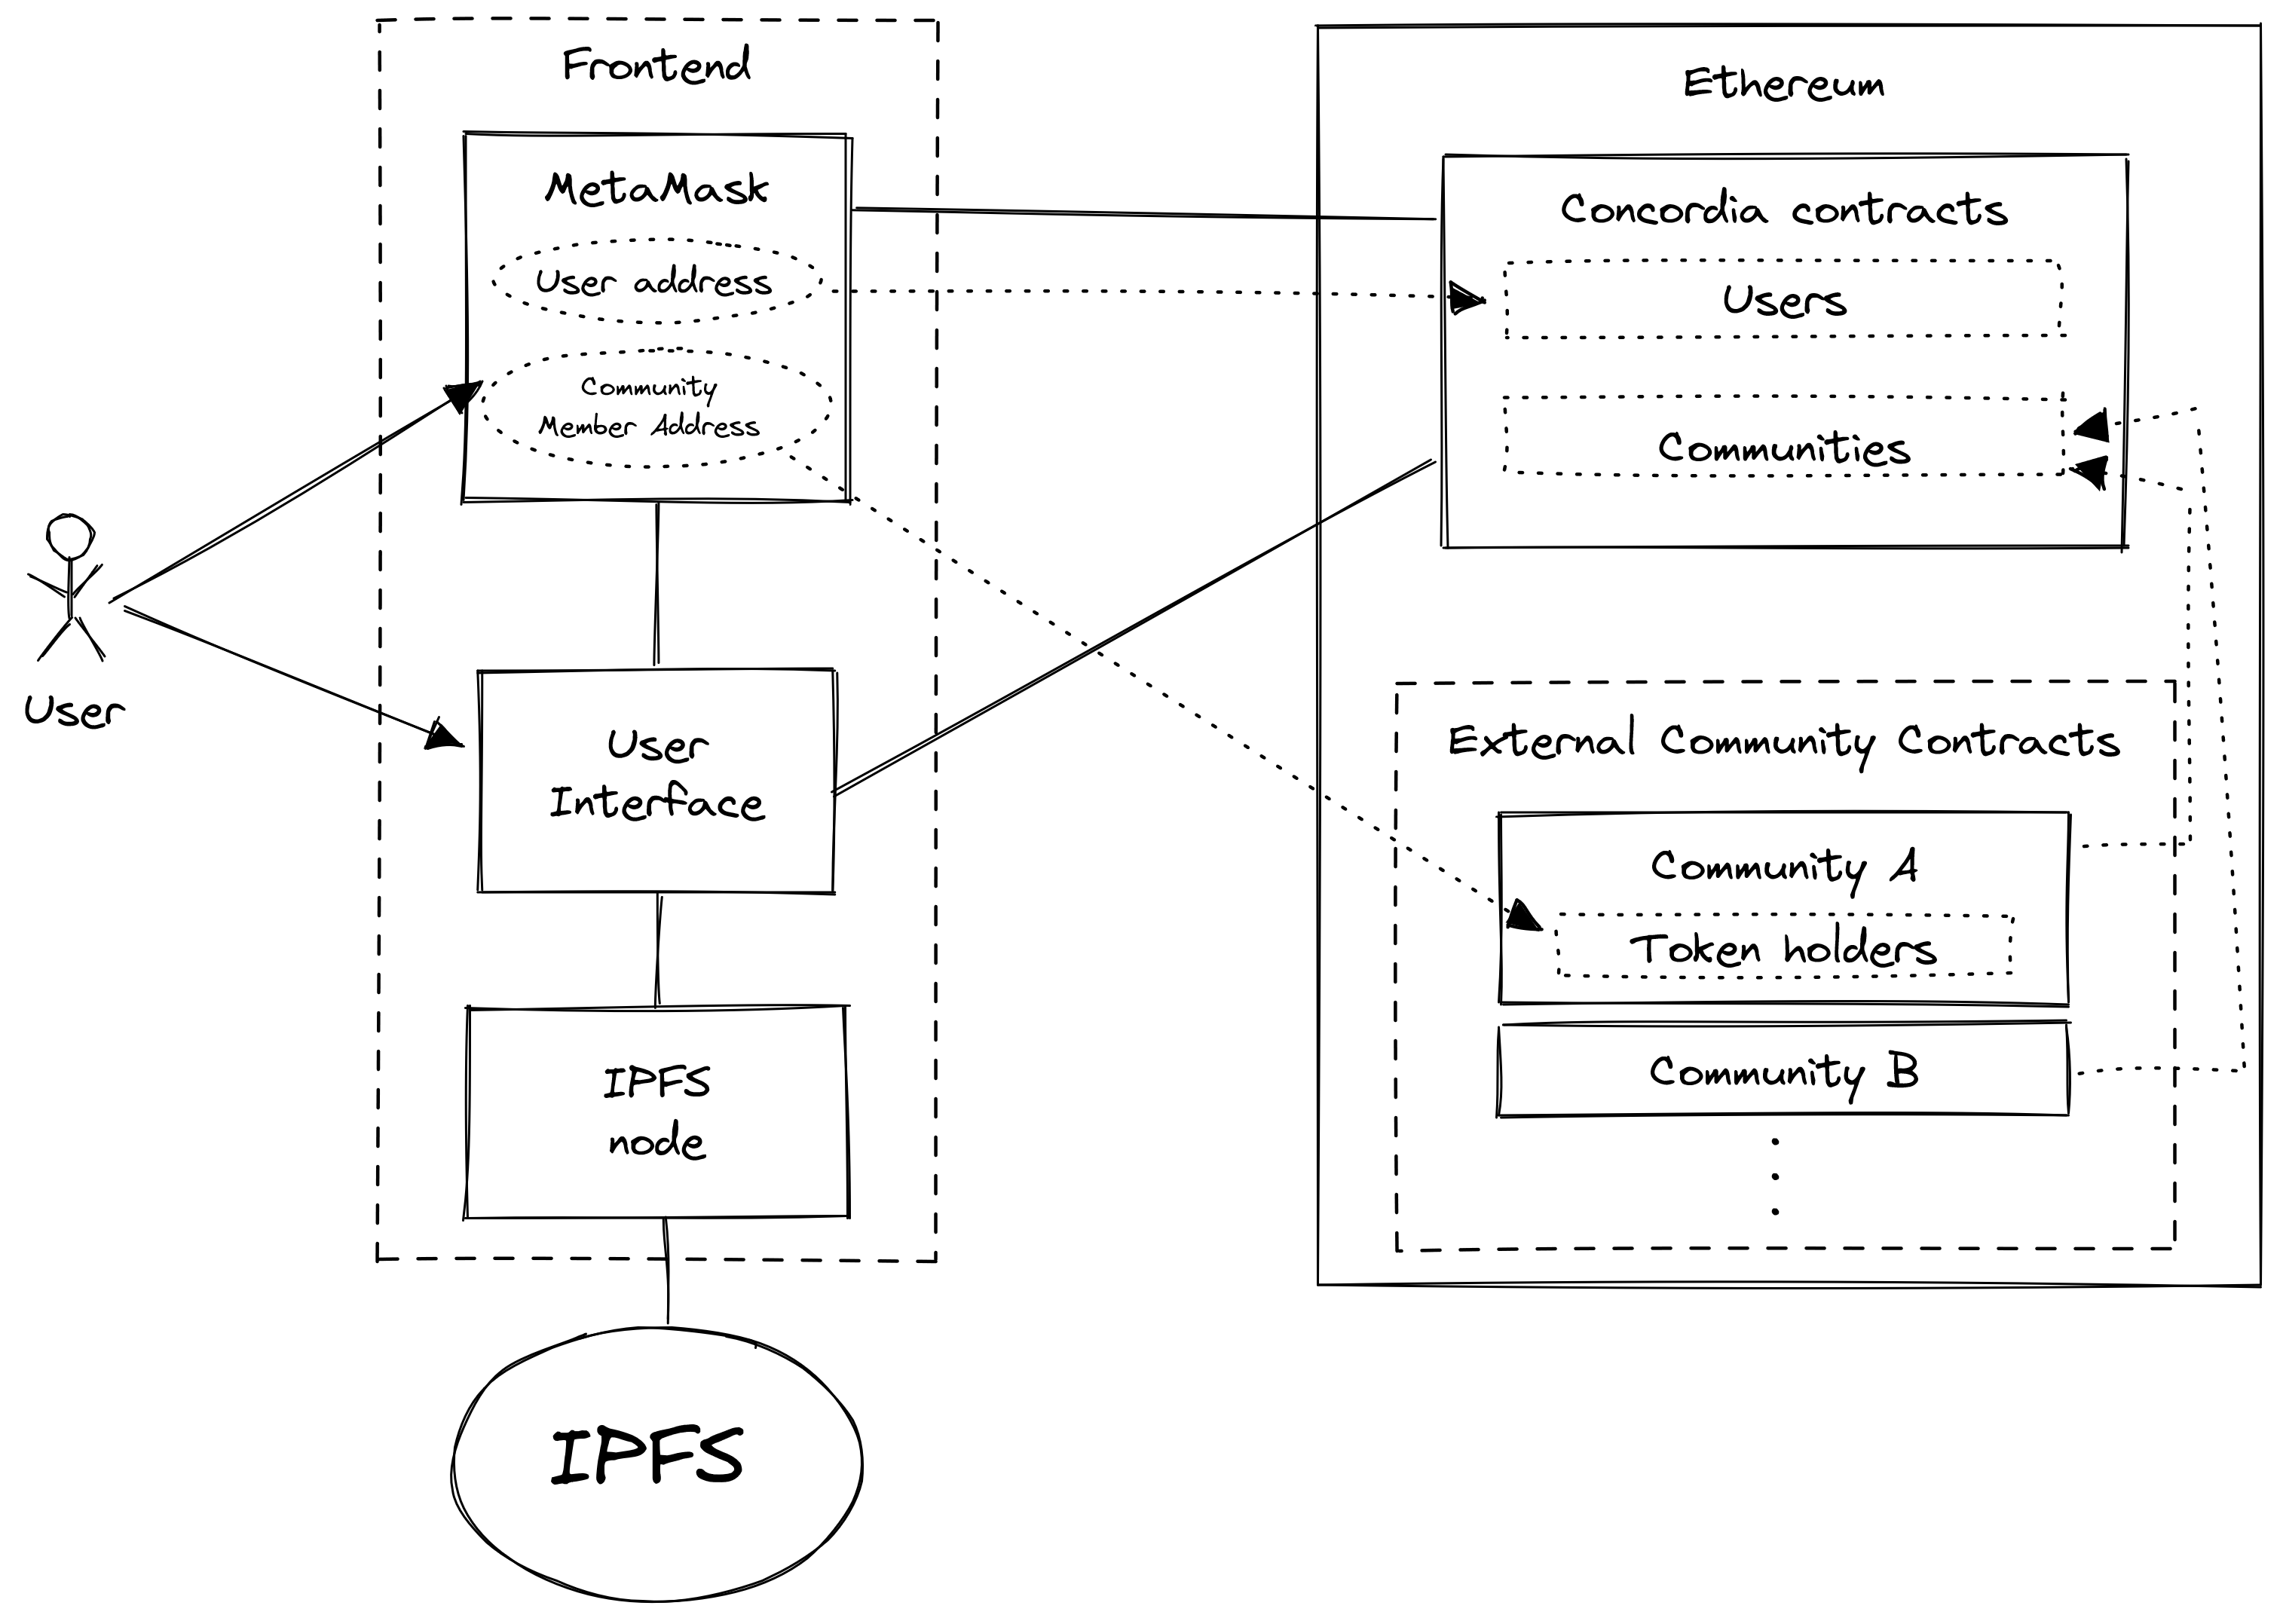
\includegraphics[width=\textwidth]{assets/figures/chapter-3/3.7.architecture-design}
    \caption{Αρχιτεκτονική του συστήματος (στάδιο σχεδίασης)}
\end{figure}

\vspace{\baselineskip}

Αξίζει να σημειωθούν τα εξής:

\begin{itemize}
    \item Ο κώδικας του frontend εκτελείται αποκλειστικά στο σύστημα του χρήστη, χωρίς να απαιτείται κάποιος εξυπηρετητής. Δηλαδή, ο χρήστης αρκεί απλά να έχει τον κώδικα αποθηκευμένο στον υπολογιστή του.
    \item Ο χρήστης αλληλεπιδρά άμεσα με το UI και το MetaMask. Το MetaMask αποτελεί browser add-on, το οποίο διαχειρίζεται τα ιδιωτικά κλειδιά Ethereum του χρήστη και πραγματοποιεί τις συναλλαγές του τελευταίου με τα smart contract. Στην προκειμένη περίπτωση, περιέχει τα κλειδιά που σχετίζονται αφενός με τη διεύθυνση με την οποία ο χρήστης εγγράφεται στην πλατφόρμα, αφετέρου με τις διευθύνσεις που περιέχουν τα token των κοινοτήτων στις οποίες ανήκει και έχει δικαιώματα ψήφου.
    \item Στο frontend εκτελείται στο παρασκήνιο ένας κόμβος για το IPFS. Αυτός συνδέεται με άλλους κατάλληλους κόμβους, διαμοιράζοντας τον κύριο όγκο των δεδομένων της εφαρμογής (π.χ. του περιεχομένου των μηνυμάτων).
    \item Τέλος, στο Ethereum blockchain υπάρχουν τόσο τα contract της εφαρμογής, όσο και τα εξωτερικά contract που παρέχουν τα token των κοινοτήτων. Τα μεν λειτουργούν ως το σημείο αναφοράς της εφαρμογής, επί του οποίου εκτελούνται οι ενέργειες και αποθηκεύονται οι μεταβλητές που είναι απολύτως απαραίτητες για τη λειτουργία της πλατφόρμας (π.χ. εγγεγραμμένοι χρήστες, δημιουργημένες κοινότητες). Τα δε δημιουργούνται από εξωτερικές οντότητες, οι οποίες ορίζουν κατά τη βούλησή τους τον ακριβή τρόπο δημιουργίας και διαμοιρασμού των token τους στους χρήστες.
\end{itemize}
\section{Προδιαγραφή μεθόδου υλοποίησης και χρονοπρογραμματισμός} \label{section:3-8-implementation-methodology-specification}

% TODO: remove feeless and reputation from cycles, add communities

\subsection{Προδιαγραφή κύκλων}

Εποπτικά, η διαδικασία της υλοποίησης περιγράφεται ως εξής:

% TODO: insert revamped diagram

\subsection{Πρώτη φάση}

% Παλιό από Drive
Στήνεται ένα Ethereum Private Network ως βάση πάνω στην οποία θα δουλέψουμε. Πάνω σε αυτό γράφουμε τα contracts που θα είναι υπεύθυνα για διεκπεραίωση ή μη των posts.
Στη συνέχεια αναπτύσσεται ο απαραίτητος κώδικας που υλοποιεί το posting χρησιμοποιώντας τις βιβλιοθήκες που δίνονται από το IPFS για την επικοινωνία μεταξύ των κόμβων του δικτύου και αυτές που δίνονται από τη BigChainDB για την αποθήκευση των πληροφοριών με διανεμημένο τρόπο.
Γίνονται δοκιμές για την εξακρίβωση της σωστής λειτουργίας του αποτελέσματος και διορθώνονται τυχόν λάθη στο κώδικα.

\subsection{Δεύτερη φάση}

% Παλιό από Drive
Υλοποιείται το δικαίωμα ψήφου και posting χωρίς fees. Αυτό γίνεται μέσω δύο contracts που θα δημιουργούν δύο διαφορετικά tokens (voting token, feeless token) και θα τα αποδίδουν στον εκάστοτε χρήστη που πρέπει να πάρει το δικαίωμα.
Αναπτύσσεται κώδικας που να υλοποιεί τη διαδικασία ψηφοφορίας.
Γίνονται δοκιμές για την εξακρίβωση της σωστής λειτουργίας του αποτελέσματος και διορθώνονται τυχόν λάθη στο κώδικα. Σε αυτή τη φάση η απόδοση των tokens θα γίνει χειροκίνητα για το σκοπό της δοκιμής.

\subsection{Τρίτη φάση}

% Παλιό από Drive
Υλοποιείται ένα σύστημα απόδοσης εμπιστοσύνης (ΣΑΠ).
Αναπτύσσονται τα contracts που είναι απαραίτητα για τη λειτουργία του ΣΑΠ καθώς και για την αυτόματη απόδοση feeless token στους trusted χρήστες.
Γίνονται δοκιμές για την εξακρίβωση της σωστής λειτουργίας του αποτελέσματος και διορθώνονται τυχόν λάθη στο κώδικα.
Εφόσον η εφαρμογή περάσει το στάδιο των δοκιμών είναι έτοιμη για alpha deployment, είναι δηλαδή έτοιμη για χρήση από το κοινό, υπολείπονται όμως χαρακτηριστικά που είναι ιδιαίτερα θεμιτά αλλά όχι απαραίτητα για τη λειτουργία.

\subsection{Τέταρτη φάση}

% Παλιό από Drive
Αναπτύσσεται ο κώδικας του (μοναδικού) συγκεντρωτικού τμήματος του συστήματος το οποίο ανήκει στο δεύτερο κομμάτι - του UAS: Έτσι αυτοματοποιείται η διαδικασία απόδοσης των token, που στην προηγούμενη φάση έγινε χειροκίνητα.
Γίνονται δοκιμές για την εξακρίβωση της σωστής λειτουργίας του αποτελέσματος και διορθώνονται τυχόν λάθη στο κώδικα.
Εφόσον η εφαρμογή περάσει το στάδιο των δοκιμών είναι έτοιμη για ένα beta deployment, ώστε να γίνει πιο ευρύς έλεγχος από μία ομάδα δοκιμών και να παρθεί feedback για την εμπειρία χρήστη.

Για το τελικό deployment θα μπορούσε να τεθεί ως στόχος η κατά το δυνατόν μείωση των τελών για τη λειτουργία της πλατφόρμας, ανεπτυγμένα χαρακτηριστικά επικοινωνίας όπως δόμηση των συζητήσεων σε κατηγορίες, προφίλ χρηστών και άλλα χαρακτηριστικά ευκολίας χρήσης.

